% 
% Author: Thomas C. Hales
% Affiliation: University of Pittsburgh
% email: hales@pitt.edu
%
% latex format

% History.  File started Jan 12, 2011
% 
%% 

\documentclass{llncs}
\usepackage{verbatim}
\usepackage{graphicx}
\usepackage{amsfonts}
\usepackage{amscd}
\usepackage{amssymb}
\usepackage{amsmath}

\usepackage{alltt}
\usepackage{rotating}
\usepackage{floatpag}
 \rotfloatpagestyle{empty}
%\usepackage{amsthm}
\usepackage{graphicx}
\usepackage{multind}\ProvidesPackage{multind}
\usepackage{times}

% my additions
\usepackage{verbatim}
\usepackage{latexsym}
\usepackage{crop}
\usepackage{txfonts}
\usepackage[hyphens]{url}
\usepackage{setspace}
\usepackage{ellipsis} % 
% http://www.ctan.org/tex-archive/macros/latex/contrib/ellipsis/ellipsis.pdf 
%\setstretch{2}  % for double spacing

% fonts
\usepackage[mathscr]{euscript} % powerset.
\usepackage{pifont} %ding
\usepackage[displaymath]{lineno}
\usepackage{rotating}

%%\usepackage{fancyhdr}
%%\usepackage{mparhack}
%%\usepackage{edmargin} %endnotes


%\def\szincludegraphics[#1]#2{%
%\includegraphics[#1]{#2}}


% automatically generate revision number by
% svn propset svn:keywords "LastChangedRevision" turing.tex
\def\svninfo{{\tt
  filename: turing.tex\hfill\break
  PDF generated from LaTeX sources on \today; \hfill\break
  Repository Root: https://flyspeck.googlecode.com/svn \hfill\break
  SVN $LastChangedRevision: 1552 $
  XX Graphics and table permissions pending
  }
  }
%-%

% Math notation.
\def\op#1{{\hbox{#1}}} 
\def\tc{\hbox{:}}
\newcommand{\ring}[1]{\mathbb{#1}}
\def\amp{\text{\&}}
\def\bq{\text{\tt {`}\,}}
\def\true{\text{true}}
\def\false{\text{false}}
% Flags


%%%%%%%%%%%%%%%%%%%%%%%%%%%%%%%%%%

\begin{document}

\title{Mathematics in the Age of the Turing Machine}
\author{Thomas C. Hales\thanks{{Research supported in part by the Benter Foundation.}}}
\institute{University of Pittsburgh\\
\email{hales@pitt.edu}}
\maketitle



\section*{}

\begin{figure}[h!]
  \centering
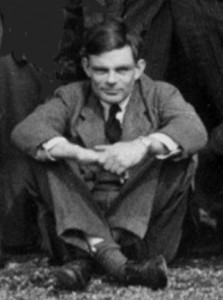
\includegraphics[scale=0.8]{alan-turing-223x300.jpg}
  \caption{Alan Turing}
\end{figure}
% image from http://www.heideschwaetzer.de/digitale-fundstuecke/beweis-eine-million-dollar-belohnung/
% XX permissions needed.


{

\narrower

\it

``And when it comes to mathematics, you must realize that this is the human mind
at the extreme limit of its capacity.'' (H. Robbins) 

\smallskip
\noindent
``\ldots so reduce the use of
the brain and calculate!'' (E. W. Dijkstra)  

\smallskip
\noindent
``The fact that a brain {\it can} do it seems to suggest that the
difficulties [of trying with a machine] may not really be so bad as they now
seem.''  (A. Turing)
% Essential Turing page 504, 

}

\newpage

\section{Automating Calculation}

\subsection{a panorama of the status quo}

Where stands the mathematical endeavor?

In 2012, many mathematical utilities are reaching consolidation.  It
is an age of large aggregates and large repositories of mathematics:
the arXiv, Math Reviews, and euDML, which promises to aggregate the
many European archives such as Zentralblatt Math and Numdam.  Sage
aggregates dozens of mathematically oriented computer
programs under a single Python-scripted front-end.

% XX check dozens, hundreds??
% XX cite euDML http://www.eudml.eu

Book sales in the U.S. have been dropping  for the past several years. 
%\cite{BK11}
% ``Sales of print books in the U.S. peaked in   2005 and have been in steady decline since.''
Instead, online sources -- {\it Wikipedia, Math Overflow, Planet
  Math}, Weinstein's {\it Math World}, and Sloane's {\it Online
  Encyclopedia of integer sequences} -- are rapidly becoming students'
preferred math references. The Polymath blog organizes massive
mathematical collaborations.  Other blogs organize previously isolated
researchers into new fields of research.  The slow, methodical
deliberations of referees in the old school are giving way;
% like a body with high
%inertia, no external energy source, and heavy friction.  Meanwhile,
now in a single stroke,  Tao blogs, gets feedback, and publishes.



Machine Learning is in its ascendancy.  {\it LogAnswer} and {\it
  Wolfram Alpha} answer our elementary questions about the
quantitative world; {\it Watson} our {\it Jeopardy} questions. {\it
  Google Page} ranks our searches by calculating the largest eigenvalue of the largest matrix
the world has ever known.  {\it Deep Blue} plays our chess
games. The million-dollar-prize-winning {\it Pragmatic Chaos}
algorithm enhances our {\it Netflix searches}.  The major proof
assistants now contain tens of thousands of formal proofs that are
being mined for hints about how to prove the next generation of
theorems.

Mathematical models and algorithms rule the quantitative world.
%``Without [applied mathematics] we would have no internet, no scanner
%at store counters, no airplane flights or space exploration, no global
%warming measurements, and of course no baseball
%statistics''~\cite{Pi2011}.  
Without applied mathematics, we would be bereft of Shor's
factorization algorithm for quantum computers, Yang-Mills theories of
strong interactions in physics, invisibility cloaks, Radon transforms
for medical imaging, models of epidemiology, risk analysis in
insurance, stochastic pricing models of financial derivatives, RSA
encryption of sensitive data, Navier-Stokes modeling of fluids, and
models of climate change.
%As Pitici reminds us, without applied math, ``no
%internet, no scanner at store counters, \dots no space exploration
%\dots and of course no baseball statistics''~\cite{Pi11}.  
Without it, entire fields of engineering from Control Engineering to
Operations Research would close their doors.  The early icon of
mathematical computing, Von Neumann, divided his final years between
meteorology and hydrogen bomb calculations.
% Reference Birds and Frogs essay of Dyson.
Today, applications fuel the
economy: in 2011 rankings, the first five of the ``10 best jobs'' are
math or computer related: software engineer, mathematician, actuary,
statistician, and computer systems analyst~\cite{CC11}.  
%\footnote{Yet
%  the popular media still portrays the mathematician as one who writes
%  formulas on windows and mirrors in a crazed frenzy, rather than as a
%  driver of the global economy.}

% CC11 http://www.careercast.com/jobs-rated/10-best-jobs-2011

% http://money.cnn.com/magazines/moneymag/bestjobs/2010/snapshots/1.html

% LogAnswer http://www.uni-koblenz.de/~bpelzer/publications/FGHP08_IJCAR08_prel.pdf
% http://en.wikipedia.org/wiki/Netflix_Prize





\bigskip

Computers have rapidly become so pervasive in mathematics that future
generations may look back to this day as a golden dawn.  A
comprehensive survey is out of the question.  It would almost be like
asking for a summary of applications of symmetry to mathematics.
Computability -- like symmetry -- is a wonderful structural property
that some mathematical objects possess that makes answers flow more
readily wherever it is found.  This section gives many examples that
give a composite picture of computers in mathematical research,
showing that computers are neither the panecea that the public at
large might imagine, nor the evil that the mathematical purist might
fear.  I have deliberated selected many examples from pure
mathematics, partly because of my own background and partly to correct
the conventional wisdom that couples computers with applied
mathematics and blackboards with pure mathematics.


\subsection{Birch and Swinnerton-Dyer conjecture}

I believe that the Birch and Swinnerton-Dyer conjecture is the deepest
conjecture ever to be formulated with the help of a computer~\cite{BSD}.  The
Clay Institute has offered a one-million dollar prize to anyone who
settles it.

Let $E$  be an elliptic curve defined by
an equation $y^2 = x^3 + a x + b$ 
over the field of rational
numbers.  Motivated by related quantities in Siegel's work on quadratic forms, Birch and Swinnerton-Dyer set out to estimate the quantity
\begin{equation}\label{eqn:np}
\prod {N_p/p},
\end{equation}
where $N_p$ is the number of rational points on $E$ modulo $p$, and
the product extends over primes $p\le P$~\cite{Bir}.  Performing
experiments on the EDSAC II computer at the Computer laboratory at Cambridge University during the years 1958--1962, they observed that as $P$ increases, the products (\ref{eqn:np})
grow asymptotically in $P$ as 
\[
c(E) \log^r P,
\]
for some constant $c$, where $r$ is the Mordell-Weil rank of $E$; that
is, the maximum number of independent points of infinite order in the
group $E(\ring{Q})$ of rational points.  Following the suggestions of
Cassels and Davenport, they reformulated this numerical asymptotic law in
terms of the zeta function $L(E,s)$ of the elliptic curve.  Thanks to the work of Wiles
and subsequent extensions of that
work, it is known that $L(E,s)$ is an entire function of the complex
variable $s$.  The Birch and Swinnerton-Dyer conjecture asserts that
the rank $r$ of an elliptic curve over $\ring{Q}$ is equal to the
order of the zero of $L(E,s)$ at $s=1$.

A major (computer-free) recent theorem establishes that the Birch and Swinnerton-Dyer
conjecture holds for a positive proportion of all elliptic curves over
$\ring{Q}$~\cite{BS:2010}.  This result, although truly spectacular, is
mildly misleading in the sense that the elliptic curves of high rank rarely
occur but pose the greatest difficulties.





\subsection{Sato-Tate}

% Math content checked Sep 2, 2011.

\begin{figure}[h!]
  \centering
\includegraphics[scale=0.25]{sato.pdf}
  \caption{Data leading to the Sato-Tate conjecture.}
\label{fig:st}
\end{figure}

% Sato-Tate:
% Sato's calc: graphic, http://www.math.ou.edu/~rschmidt/satotate/ST2.pdf
% publish this.
%% Sato's history of computation:
%% http://www.math.ou.edu/~rschmidt/satotate/page5.html


The Sato-Tate conjecture is another major conjecture about elliptic
curves that was discovered by computer.  If $E$ is an elliptic curve
with rational coefficients
\[
y^2 = x^3 + a x + b,
\]
then the number of solutions modulo a prime number $p$ (including the
point at infinity) has the form
\[
1 + p - 2\sqrt{p}\cos\theta_p.
\]
for some real number $0\le \theta_p\le \pi$.  In 1962, Sato,
Nagashima, and Namba made calculations  of $\theta_p$ on a Hitachi
HIPAC 103 computer to understand how these numbers are distributed as
$p$ varies for a fixed elliptic curve $E$~\cite{Sch}.  By the spring of 1963, the
evidence suggested  $\sin^2\theta$ as a good fit of the data (Figure~\ref{fig:st}).
That is, if $P(n)$ is is the set of the first $n$ primes, and
$f:[0,\pi]\to\ring{R}$ is any smooth test function, then for large
$n$,
\[
\frac{1}{n}\sum_{p\in P(n)} f(\theta_p) \quad\hbox{ tends to }\quad
\frac{2}{\pi}\int_0^\pi f(\theta)\,\sin^2\theta\,d\theta.
\]
The Sato-Tate conjecture (1963) predicts that this same distribution is
obtained, no matter the elliptic curve, provided the curve does not
have complex multiplication.  Tate, who arrived at the conjecture
independently, did so without computer calculations.

Serre interpreted Sato-Tate as a generalization of Dirchlet's
theorem on primes in arithmetic progression, and gave a proof strategy
of generalizing the analytic properties of $L$-functions used in
the proof of Dirichlet's theorem~\cite{Se68}.  Indeed, a complete proof of Sato-Tate
conjecture has now been found and is based on (extremely deep)
analytic properties of $L$-functions~\cite{Car:Bourbaki}.
The proof of the Sato-Tate conjecture and its generalizations has been
one of the most significant recent advances in number theory.







\subsection{transcient uses of computers}

It has become common for problems mathematics to be first verified by
computer and later confirmed without them.  Some examples are
the construction of sporadic groups, counterexamples to a conjecture
of Euler, the proof of the Catalan conjecture, and the discovery of a formula
for the binary digits of $\pi$.

Perhaps the best known example is the construction sporadic groups as
part of the monumental classification of finite simple groups.  The
sporadic groups are the $26$ finite simple groups that do not fall into
natural infinite families.  For example,  Lyons (1972) predicted
the existence of a sporadic group of order
\[
2^ 8\cdot 3^7\cdot 5^6\cdot  7\cdot 11 \cdot 31 \cdot 37 \cdot 67.
\]
In 1973, Sims proved the existence of this group in a long unpublished
manuscript that relied on many specialized computer programs.  By 1999
, the calculations had become standardized in group theory packages,
such as GAP and Magma~\cite{HS99}.  Eventually, computer-free
existence and uniqueness proofs were found~\cite{MParker},
\cite{AS92}.

%%T Cite ref TR0416 (Sims 1999), for the 1973 calculations
%%T http://dimacs.rutgers.edu/~havas/TR0416.pdf  (Havas and Sims, 1999) on laptop.
%% http://en.wikipedia.org/wiki/Lyons_group

Another problem in finite group theory with a computational slant is
the inverse Galois problem: is every subgroup of the symmetric group
$S_n$ the Galois group of a polynomial of degree $n$ with rational
coefficients?  In the 1980s Malle and Matzat used computers to realize
many groups as Galois groups~\cite{MM}, but with an infinite list of
finite groups to choose from, non-computational ideas have been more
fruitful, such as Hilbert irreducibility, rigidity, and automophic
representations~\cite{KLS}.

\smallskip

Euler conjectured (1769) that a fourth power cannot be the sum of
three positive fourth powers, that a fifth power cannot be the sum of
four positive fifth powers, and so forth.  In 1966, a computer search
\cite{LP66} on a CDC 6600 mainframe uncovered a counterexample
\[
27^5 + 84^5 + 110^5 + 133^5 = 144^5,
\]
which can be checked by hand (I dare you).  The two-sentence
announcement of this counterexample qualifies as one of the shortest
mathematical publications of all times.  Twenty years later, a more
subtle computer search gave another counterexample~\cite{Elkies88}:
\[
2682440^4 + 15365639^4 + 18796760^4 = 20615673^4.
\]

%% http://en.wikipedia.org/wiki/Euler's_sum_of_powers_conjecture

\smallskip

The Catalan conjecture (1844) asserts that the only solution to the equation
\[
x^m - y^n = 1,
\]
in positive integers $x,y,m,n$ with exponents $m,n$ greater than $1$
is the obvious
\[
3^2 - 2^3 = 1.
\]
That is, $8$ and $9$ are the only consecutive positive perfect powers.
By the late 1970s, Baker's methods in diophantine analysis had reduced
the problem to an astronomically large and hopelessly infeasible finite
computer search.  Mih\u ailescu's proof (2002) of the Catalan
conjecture made light use of computers (a one-minute calculation), and
later the computer calculations were entirely eliminated~\cite{Mih},~\cite{TM03}.

\smallskip

%% computer use in Catalan ... Bulletin article, TAUNO METS... on laptop drive. May directory.
%% eliminated in Steiger article on laptop drive.  May directory.

Bailey, Borwein, and Plouffe found an algorithm for calculating the
$n$th binary digit of $\pi$ directly: it jumps straight to the $n$th
digit without first calculating any of the earlier digits.  They
understood that to design such an algorithm, they would need an
infinite series for $\pi$ in which powers of $2$ controlled the
denominators.  They did not know of any such formula, and made a
computer search (using the PSLQ lattice reduction algorithm) for any
series of the desired form.  Their search unearthed a numerical
identity
\[
\pi = \sum_{n=0}^\infty 
\left(
\frac{4}{8n+1} - \frac{2}{8n+4} - \frac{1}{8n+5} - \frac{1}{8n+6}
\right) 
\left(\frac{1}{16}\right)^n,
\]
which was then rigorously proved and used to implement their
binary-digits algorithm.

% XX needs citation.

% make the "denominators contained powers of 2" more precise.
% http://www.andrews.edu/~calkins/physics/Miracle.pdf

%\subsection{computer assisted discovery of conjectures}


\subsection{Rogers-Ramanujan identities}

The famous Rogers-Ramanujan identities
\[
1 + \sum_{k=1}^\infty \frac{q^{k^2+a k}}{(1-q)(1-q^2)\cdots (1-q^k)} = 
\prod_{j=0}^\infty \frac{1}{(1-q^{5j+a+1})(1- q^{5j - a +4})},
\qquad a = 0,1.
\]
can now be proved by an almost entirely mechanical procedure from
Jacobi's triple product identity and the $q$-WZ algorithm of Wilf and
Zeilberger that checks identities of $q$-hypergeometric finite
sums~\cite{PP94}.   Knuth's foreward to a book
on the WZ method opens, ``Science is what we understand well enough to
explain to a computer. Art is everything else we do.'' Through the WZ
method, many summation identities have become a science~\cite{PWZ}.


\subsection{packing  tetrahedra}

Aristotle erroneously believed that regular tetrahedra tile space:
``It is agreed that there are only three plane figures which can fill
a space, the triangle, the square, and the hexagon, and only two
solids, the pyramid and the cube''~\cite{Aristotle}.  However,
centuries later, when the dihedral angle of the regular tetrahedron
was calculated:
\[
\arccos(1/3) \approx 1.23 < 1.25664 \approx 2\pi/5,
\]
it was realized that a small gap is left when five regular tetrahedra
are grouped around a common edge (Figure~\ref{fig:gap}).  In 1900, in his famous list of
problems, Hilbert asked ``How can one arrange most densely in space an
infinite number of equal solids of given form, e.g., spheres with
given radii or regular tetrahedra \dots?''

\begin{figure}[h!]
  \centering
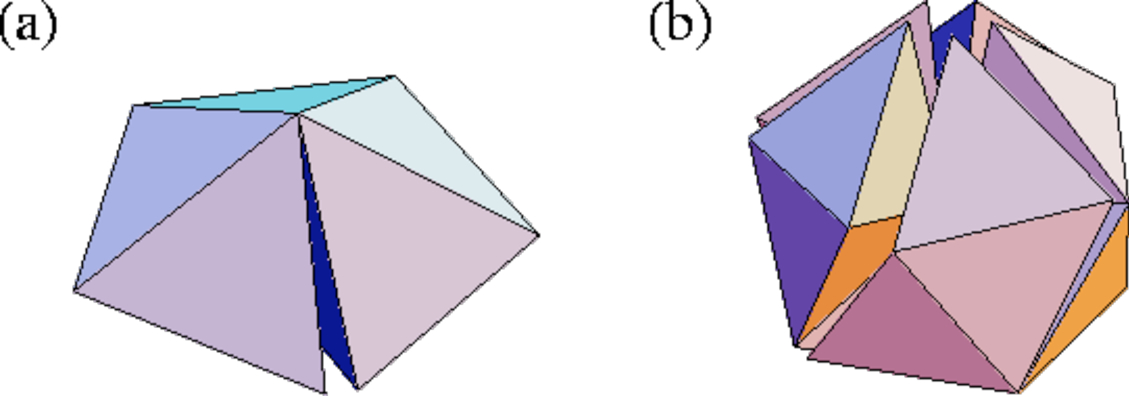
\includegraphics[scale=0.3]{tetrahedral_defect.pdf}
  \caption{Regular tetrahedra fail to tile space.}
\label{fig:gap}
\end{figure}
% image from http://physchem.ox.ac.uk/~doye/jon/structures/Morse/paper/node3.html
% XX permissions still needed.

Aristotle notwithstanding, until recently, no arrangements of regular
tetrahedra with high density were known to exist.  In 2000, Betke and
Henk developed an efficient computer algorithm to find the densest
lattice packing of a general convex body~\cite{BH2000}.  This opened
the door to experimentation~\cite{Conway-2006}.  In rapid succession
came new record-breaking arrangements of tetrahedra, culminating in
what is now conjectured to be the best possible~\cite{Chen-2010}.
(See Figure~\ref{fig:CEG}.)  Although Chen had the panache to hand out
Dungeons and Dragons tetrahedral dice to the audience for a hands-on
modeling session during her thesis defense, the best arrangement was
found using Monte Carlo experiments.  In the numerical simulations, a
finite number of tetrahedra are randomly placed in a box of variable
shape.  The tetrahedra are jiggled as as the box slowly shrinks until
no further improvement is possible.  Now that a precise conjecture has
been formulated, the hardest part still remains: to give a proof.

\begin{figure}[h!]
  \centering
\includegraphics[scale=0.9]{CEG_tetrahedra.pdf}
  \caption{The best packing of
tetahedra is believed to be the Chen-Engel-Glotzer arrangement with density
$4000/4671\approx 0.856$.}
\label{fig:CEG}
\end{figure}
% image from Chen-2010. XX Permissions still needed.


\subsection{the Kepler conjecture}

% 


Hilbert's 18th problem asks to find dense packings of both spheres and
regular tetrahedra.  The problem of determining the best sphere
packing in three dimensions is the Kepler conjecture.  Kepler was led
to the idea of density as an organizing principle in nature by
observing the tightly packed seeds in a pomegranate.  Reflecting on
the hexagonal symmetry of snowflakes and honeycombs, by capping each
honeycomb cell with a lid of the same shape as the base of the cell,
he constructed a closed twelve-sided cell that tiles space.  Kepler
observed that the familiar pyramidal cannonball arrangement is
obtained when a sphere is placed in each capped honeycomb cell
(Figure~\ref{fig:rhombic}).  This he believed to be the densest
packing.

\begin{figure}[h!]
  \centering
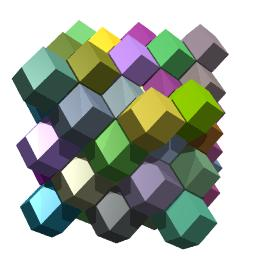
\includegraphics[scale=0.5]{Rhombic_dodecahedra.jpg}
  \caption{An optimal sphere packing is obtained by placing
one sphere in each three-dimensional honeycomb cell.}
\label{fig:rhombic}
\end{figure}
% should be freely useable? XX
% graphic source: http://archinstitute.blogspot.com/2005_10_30_archive.html
% http://upload.wikimedia.org/wikipedia/commons/8/86/Rhombic_dodecahedra.jpg

L. Fejes T\'oth proposed a strategy to prove Kepler's conjecture in
the 1950s, and later he suggested that computers might be used.  The
proof, finally obtained by Ferguson and me in 1998, is one of the
most difficult nonlinear optimization problems ever rigorously solved
by computer~\cite{Hales:2005:Annals}.  The computers calculations
originally took about $2000$ hours to run on Sparc workstations.
Recent simplifications in the proof have reduced the runtime to about
$20$ hours and have reduced the amount of customized code by a factor
of more than $10$.

% to fewer
%than $10,000$ lines.%
%\footnote{Estimates of the amount of custom code in the original 1998
%  proof are over $100$ thousand lines.}
% Sean (in revision paper) say's 137,000 for Sam and 50,000 for me.
% Duplication included.

\subsection{the four-color theorem}

The four-color theorem is the most celebrated computer proof in the
history of mathematics.  The problem asserts that it is possible to
color the countries of any map with at most four colors in such a way
that contiguous countries receive different colors.  The proof of this
theorem required about $1200$ hours on an IBM 370-168 in 1976. So much has
been written about Appel and Haken's computer solution to this problem
that it is pointless to repeat it here~\cite{AH4CT}.  Let it
suffice to cite a popular account ~\cite{Wil4CT}, a sociological
perspective~\cite{Mac}, the second generation
proof~\cite{Robertson:1997:JCTB}, and the culminating formal
verification~\cite{gonthier:2008:formal}.

%but that proof was eventually
%simplfied~\cite{Robertson:1997:JCTB}, and then formally
%verified~\cite{gonthier:2008:formal}.  Now the proof of the 4CT runs
%in a few hours on an average computer.

% 4CT page 133-134 of MacKenzie, Mechanizing Proof.


\subsection{projective planes}

A finite projective plane of order $n>1$ is defined to be a set of
$n^2 + n + 1$ lines and $n^2 + n+ 1$ points with the following
properties:
\begin{enumerate}
\item Every line contains $n+1$ points;
\item Every point is on $n+1$ lines;
\item Every two distinct lines have exactly one point of intersection;
\item Every two distinct points lie on exactly one line.
\end{enumerate}

\begin{figure}[h!]
  \centering
\includegraphics[scale=0.8]{110505-WikipediaFanoPlane.jpg}
  \caption{The Fano plane is a finite projective plane of order $2$.}
\label{fig:P2}
\end{figure}
% should be freely useable? XX
% http://www.log24.com/log/pix11A/110505-WikipediaFanoPlane.jpg = copy of
% http://en.wikipedia.org/wiki/File:Fano_plane.svg

The definition is an abstraction of properties that evidently
hold for $\ring{P}^2(\ring{F}_q)$, the projective plane over a finite
field $\ring{F}_q$, with $q=n$, for any prime power $q$.  In
particular, a finite projective plane exists whenever $n$ is a positive power of a prime
number (Figure~\ref{fig:P2}).

The conjecture is that every finite projective plane
of order $n>1$ is a prime power.  The smallest integers $n>1$
that are {\it not} prime powers are
\[
6,~10,~12,~14,~15,~\dots
\]
The brute force approach to this conjecture is to eliminate each of
these possibilities in turn.  The case $n=6$ was settled in 1938.
Building on a number of theoretical advances~\cite{MST}, Lam eliminated the case
$n=10$ in 1989, in one of the most difficult computer proofs in
history~\cite{Lam89}.  This calculation was executed over
a period of years on multiple machines and eventually totaled about 2000
hours of Cray-1A time.  

Unlike the computer proof of the four-color theorem, the
projective plane proof has never received independent verification.
Because of the possibilities of programming errors and soft errors
(see Section~\ref{sec:soft}), Lam is unwilling to call his result a
proof.  He writes, ``From personal experience, it is extremely easy to
make programming mistakes. We have taken many precautions, 
\dots
%including
%the use of two different programs to cross check selective sample
%cases and the checking of internal consistency when isomorphism
%testing is performed. 
Yet, I want to emphasize that this is only an
experimental result and it desperately needs an independent
verification, or better still, a theoretical
explanation''~\cite{LamS}.


Recent speculation at {\it Math Overflow} holds that the next case,
$n=12$, remains solidly out of computational reach~\cite{Horn}.

%% http://mathoverflow.net/questions/38632/projective-plane-of-order-12


\subsection{hyperbolic manifolds}

Computers have helped to resolve a number of open conjectures about
hyperbolic manifolds (defined as complete Riemannian manifolds with
constant negative sectional curvature $-1$), including the proof that
the space of hyperbolic metrics on a closed hyperbolic $3$-manifold is
contractible~\cite{GMT},~\cite{GabICM}.


\subsection{chaos theory and strange attractors}

The theory of chaos has been one of the great success stories of
twentieth century mathematics and science.   Turing\footnote{For
  early history, see \cite[p.~971]{Wolfram:NKS}. Turing vainly hoped that
  digital computers might be insulated from the effects of chaos.}
expressed the notion of chaos with these words, ``quite small errors
in the initial conditions can have an overwhelming effect at a later
time.  The displacement of a single electron by a billionth of a
centimetre at one moment might make the difference between a man being
killed by an avalanche a year later, or escaping''~\cite{Tu50}.
Later, the metaphor became a butterfly
that stirs up a tornado in Texas by flapping its wings in Brazil.

Thirteen years later, Lorenz encountered chaos as he ran weather
simulations on a Royal McBee LGP-30 computer~\cite{Lo63}.  When he
reran an earlier numerical solution with what he thought to be
identical initial data, he obtained wildly different results.  He
eventually traced the divergent results to a slight discrepancy in
initial conditions caused by rounding in the printout.  The {\it Lorenz
  oscillator} is the simplified form of Lorenz's original ordinary
differential equations.

A set $A$ is {\it attracting} if it has a neighborhood $U$ such
that
\[
A = \bigcap_{t\ge 0} f_t(U),
\]
where $f_t(x)$ is the solution of the dynamical system (in present
case the Lorenz oscillator) at time $t$ with initial condition
$x$. That is, $U$ flows towards the attracting set $A$.  Simulations
have discovered attracting sets with strange properties such as
non-integral Hausdorff dimension and the tendency for a small slab of
initial values to quickly spread throughout the attractor.

%Becoming
%imprecise, we have the notion of a strange attractor, which is an
%attractor whose Hausdorff dimension is not an integer. 

% Under the
%flow,``a tiny blob of initial values rapidly smears out over the
%entire attractor''~\cite{WT}.

% 

\begin{figure}[h!]
  \centering
\includegraphics[scale=0.7]{200px-Lorenz_attractor_boxed.png}
  \caption{The Lorenz oscillator gives one of the
most famous images of mathematics, a {\it strange attractor} in
dynamical systems.}
\label{fig:lorenz}
\end{figure}
% should be freely useable? XX
% http://en.wikipedia.org/wiki/Lorenz_attractor. (Collective Commons graphics.)


%Based on computer simulations, 
Lorenz conjectured in 1963 that his oscillator has a strange attractor
(Figure~\ref{fig:lorenz}).  In 1982, the Lax report cited soliton
theory and strange attractors as two prime examples of the ``discovery
of new phenomena through numerical experimentation,'' and calls such
discovery perhaps the most ``significant application of scientific
computing''~\cite{Lax}.  Smale, in his list of $18$ ``Mathematical
Problems for the Next Century'' made the fourteenth problem to present
a rigorous proof that the dynamics of the Lorenz oscillator is a
strange attractor~\cite{Sma98} with various additional properties that
make it a ``geometric Lorenz attractor.''

Tucker has solved Smale's fourteenth problem by
computer~\cite{Tuc02}~\cite{St00}.  One particularly noteworthy aspect
of this work is that chaotic systems, by their very nature, pose
particular hardships for rigorous computer analysis.  Nevertheless,
Tucker implemented the classical Euler method for solving ordinary
differential equations with particular care,  using interval
arithmetic to give mathematically rigorous error bounds.  Tucker has
been awarded numerous prizes for this work, including the Moore Prize
(2002) and the EMS Prize (2004).

Smale's list in general envisions a coming century in which computer
science, especially computational complexity, plays a much larger
role than during the past century. He finishes the list with the
open-ended philosophical problem  that echoes Turing: {\it
  ``What are the limits of intelligence, both artificial and human?''}


\subsection{$4/3$}
Mandelbrot's conjectures in fractal geometry have resulted in two
Fields Medals.  Here he describes the discovery of the
$4/3$-conjecture made in~\cite{ManFN}.  
``The notion that these conjectures might have been reached by pure
  thought -- with no picture -- is simply inconceivable.\dots
I had my programmer draw a very big sample [Brownian] motion and
  proceeded to play with it.''
He goes on to describe computer experiments that led him
enclose the Brownian motion into black clusters that looked to him like islands with
jagged coastlines (Figure~\ref{fig:4/3}).
%
% I was not trying to implement any
%  preconceived idea, simply actively ``fishing'' for new things.\dots
%  In order to achieve homogeneity, I decided to make the motion end
%  where it had started. The resulting motion biting its own tail
%  created a distinctive new shape I call Brownian cluster.  Next the
%  same purely aesthetic consideration led to further processing. The
%  continuing wish to eliminate extraneous complexity made me combine
%  all the points that cannot be reached from infinity without crossing
%  the Brownian cluster. Painting them in black sufficed, once again,
%  to create something quite new, resembling an island.  Instantly, it
%  became apparent that its boundary deserved to be investigated. Just
%  as 
%``\dots 
``[I]nstantly, my long previous experience with the coastlines of
  actual islands on Earth came handy and made me suspect that the
  boundary of Brownian motion has a fractal dimension equal to $4/3$''
\cite{Man}.
%  (Mandelbrot \cite{Man})
%
%}
%
%\bigskip
This conjecture, which  Mandelbrot's trained eye spotted in an instant,
took 18 years to prove~\cite{LSW01}.

\begin{figure}[h!]
  \centering
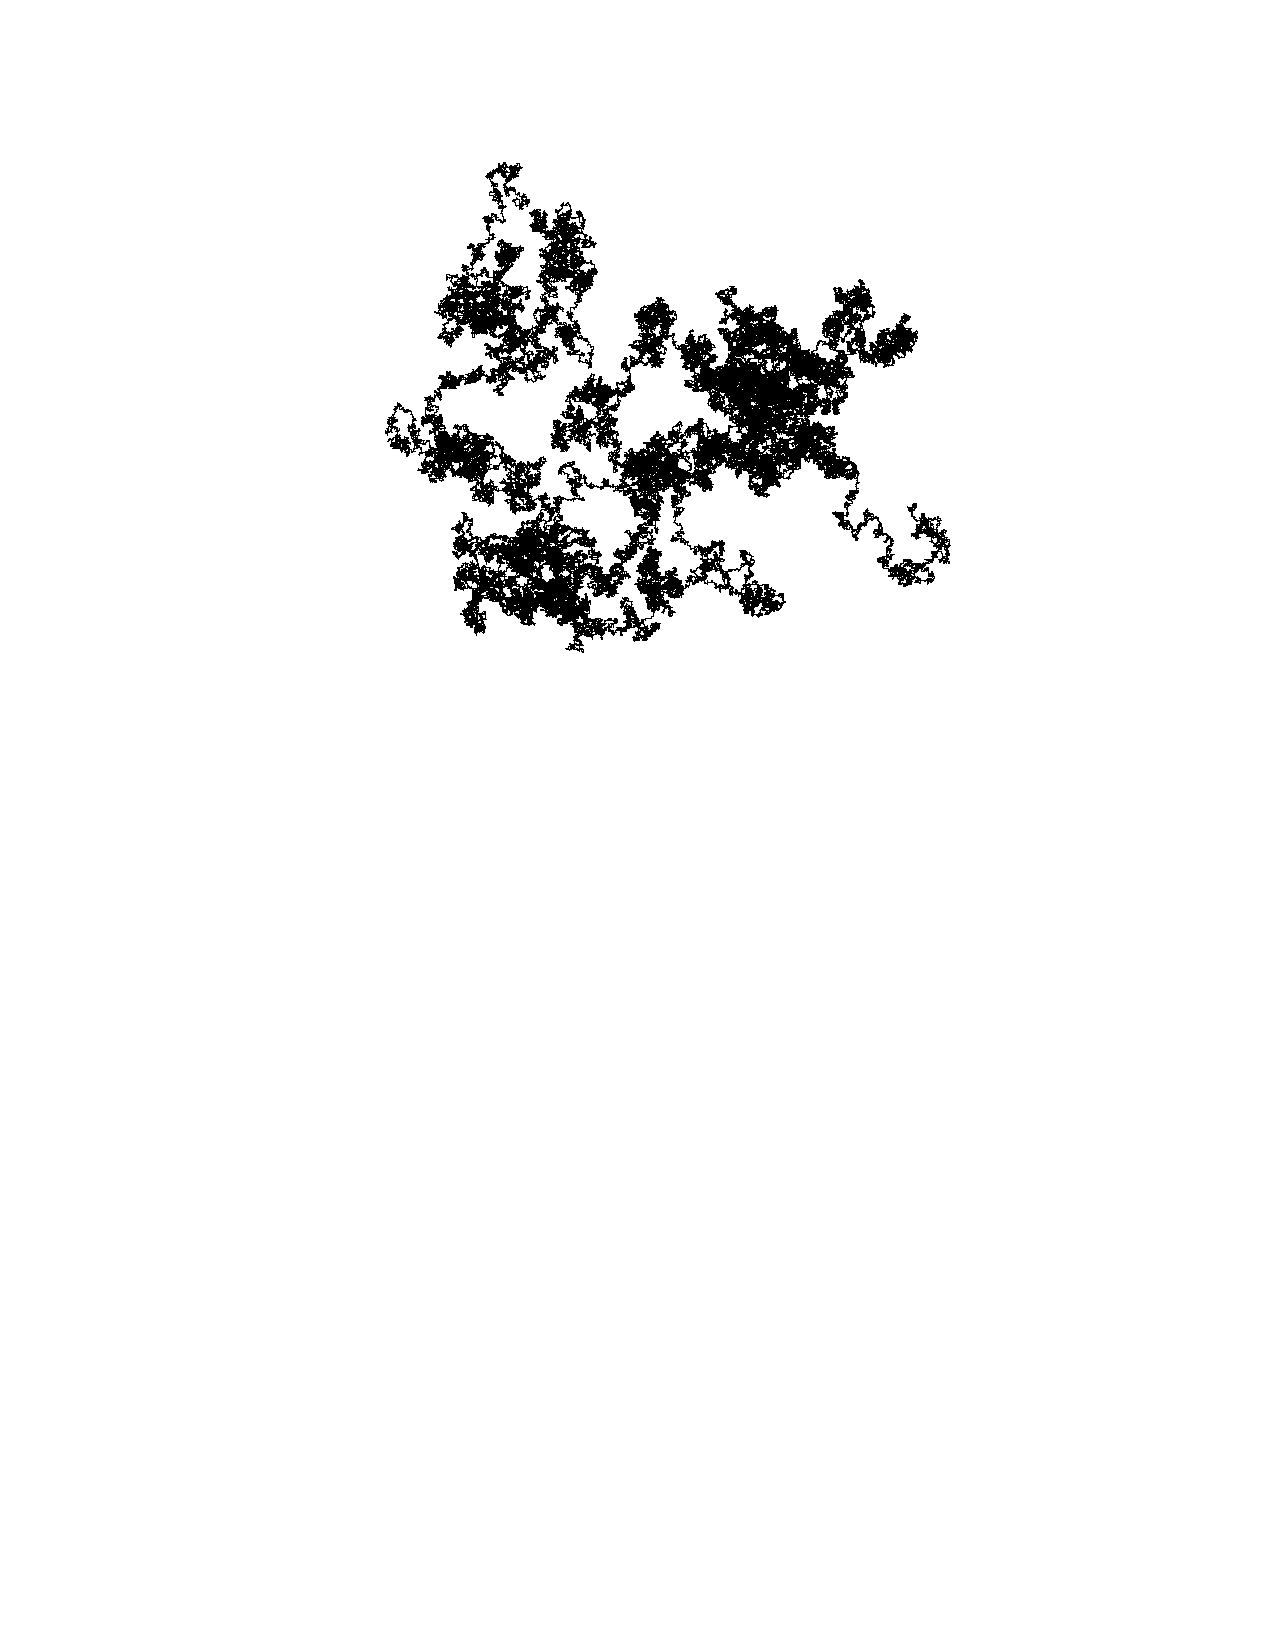
\includegraphics[scale=0.5]{brownian_motion.pdf}
  \caption{A simulation of planar Brownian motion. Mandelbrot used ``visual
inspection supported by computer experiments'' to formulate deep
conjectures in fractal geometry.}
\label{fig:4/3}
\end{figure}
% graphic source http://www.mrlonline.org/mrl/2001-008-004/2001-008-004-001.pdf
% XX permissions needed.

% Mandelbrot uses the phrase  ``visual inspection supported by computer experiments'', 
%http://users.math.yale.edu/users/mandelbrot/web_pdfs/EncycScienceAndTechnologyFractals.pdf
% use this phrase in a caption of Brownian motion image.
%
%
%Mandelbrot's 4/3 conjecture (1982), the Fractal Geometry of Nature.
%proved recently by Lawlor, Schramm, Werner.
%2001 proof.
% http://www.mrlonline.org/mrl/2001-008-004/2001-008-004-001.pdf

%% Mandelbrot quotation appears in the interview.
%% A theory of roughness.
%% http://www.edge.org/3rd_culture/mandelbrot04/mandelbrot04_index.html
%%



\subsection{sphere eversion visualization}

% http://en.wikipedia.org/wiki/Smale's_paradox

% http://torus.math.uiuc.edu/jms/Papers/isama/eversions.pdf Sullivan

%% Levy http://www.math.sunysb.edu/CDproject/OvUM/cool-links/www.geom.umn.edu/docs/outreach/oi/history.html

%%  Anthony Phillips, ``Turning a surface inside out'', Scientific American, May 1966, 112--120.

%% [Le] Silvio Levy. Making Waves: A Guide to the Ideas Behind "Outside In". AK Peters, Wellesley, MA, 1995.


Smale (1958) proved that it is possible to turn a sphere inside out
without introducing any creases.\footnote{I am fond of this example,
because The Scientific American
  article \cite{Phi66} about this theorem was my first exposure to ``real
  mathematics'' as a child.}  For a long time, this paradoxical result
defied the intuition of experts.  R. Bott, who had been Smale's
graduate advisor, refused to believe it at first.  Levy writes that
trying to visualize Smale's mathematical argument ``is akin to
describing what happens to the ingredients of a souffl\'e in minute
detail, down to the molecular chemistry, and expecting someone who has
never seen a souffl\'e to follow this `recipe' in preparing the
dish''~\cite{Le95}.

\begin{figure}[h!]
  \centering
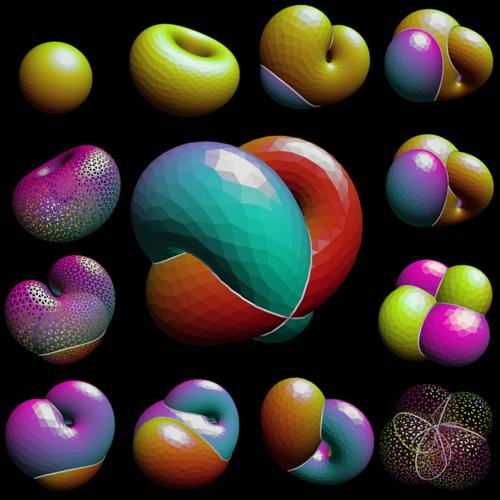
\includegraphics[scale=0.5]{bivtile.jpeg}
  \caption{Computer-generated stages of a sphere eversion.}
\label{fig:eversion}
\end{figure}

% http://new.math.uiuc.edu/optiverse/images.html graphics source, permissions needed XX.

It is better to see and taste a souffl\'e first.  The computer videos
of this theorem are spectacular.  Watch them on YouTube!  As we watch
the sphere turn inside out, our intuition grows.  The computer
calculations behind the animations of the first video (the Optiverse)
start with a sphere, half inverted and half rightside out~\cite{SFL}.  From
halfway position, the path of steepest descent of an energy functional is
used to calculate the unfolding in both directions to the round spheres,
with one fully inverted (Figure~\ref{fig:eversion}).  The second video is based on Thurston's
``corrugations''~\cite{LMM}. As the name suggests, this sphere eversion has
undulating ruffles that dance like a jellyfish, but avoids sharp
creases.   Through computers, understanding.

Speaking of Thurston, he contrasts ``our amazingly rich abilities to absorb
geometric information and the weakness of our innate abilities to convey
spatial ideas.\ldots  We effortlessly look at a two-dimensional picture
and reconstruct a three-dimensional scene, but we can hardly draw them
accurately''~\cite{Pi11}.  As more and more mathematics migrates to the computer,
there is a danger that geometrical intuition becomes buried under a logical
symbolism.

\subsection{minimal surface visualization} % (visualization)

Weber and Wolf \cite{WW11} report that the use of computer
visualization has become ``commonplace'' in minimal surface research,
``a conversation between visual aspects of the minimal surfaces and
advancing theory, each supporting the other.''  This started when
computer illustrations of the Costa surface (a particular minimal
surface, Figure~\ref{fig:costa}) in the 1980s revealed dihedral symmetries of the surface that
were not seen directly from its defining equations.  The observation
of symmetry turned out to be the key to the proof that the Costa
surface is an embedding.  The symmetries further led to a conjecture
and then proof of the existence of other minimal surfaces of higher
genus with similar dihedral symmetries.  As Hoffman wrote about his discoveries, ``The
images produced along the way were the objects that we used to make
discoveries. They are an integral part of the process of doing
mathematics, not just a way to convey a discovery made without their
use'' \cite{Hoffman}.

\begin{figure}[h!]
  \centering
\includegraphics[scale=0.4]{g1costa.jpg}
  \caption{The Costa surface launched an era of computer exploration
in minimal surface theory.}
\label{fig:costa}
\end{figure}
% http://www.math.kobe-u.ac.jp/DIVERSIONS/g1costa.jpg graphics source, XX permissions needed.



\subsection{double bubble conjecture}

Closely related to minimal surfaces are surfaces of constant mean
curvature.  The mean curvature of a minimal surface is zero; surfaces
whose mean curvature is constant are a slight generalization.  They
arise as surfaces that are minimal subject to the constraint that
they enclose a region of fixed volume.  Soap bubble films are
surfaces of constant mean curvature.  

The isoperimetric inequality asserts that the sphere minimizes the
surface area among all surfaces that enclose a region of fixed volume.
The double bubble problem is the generalization of the isoperimetric
inequality to two enclosed volumes.  What is the surface minimizing way
to enclose and separate two regions of fixed volume?  In the
nineteenth century, Boys~\cite{Boy1890} and Plateau observed
experimentally that the answer should be two partial spherical bubbles
joined along a shared flat disk (Figure~\ref{fig:double}).  The size of the shared
disk is determined by the condition that angles should be $120^\circ$
where the three surfaces meet.  This is the {\it double bubble
  conjecture}.

The first case of double bubble conjecture to be established was that
of two equal volumes~\cite{HHS95}.  The proof was a combination of conventional
analysis and computer proof.  Conventional analysis (geometric measure
theory) established the existence of a minimizer and reduced the
possibilities to a small number of figures of revolution, and
computers were to analyze each of the cases, showing in each case by
interval analysis either that the case was not a local minimizer or
that its area was strictly larger than the double bubble.  Later
theorems proved the double bubble conjecture in the general unequal
volume case without the use of computers~\cite{HMRR}.

\begin{figure}[h!]
  \centering
\includegraphics[scale=0.18]{sdb-156.jpeg}
  \caption{The optimality of this double bubble was first established by
computer, using interval analysis.}
\label{fig:double}
\end{figure}
% http://math.berkeley.edu/~hutching/pub/bubbles.html XX permissions needed.


The natural extension of the double bubble conjecture from two bubbles
to an infinite bubbly foam is the Kelvin problem.  The problem asks
for the surface area minimizing partition of Euclidean space into
cells of equal volume.  Kelvin's conjecture -- a tiling by slight
perturbations of truncated octahedra -- remained the best known
partition until a counterexample was constructed by two physicists,
Phelan and Weaire in 1993 (Figure~\ref{fig:PW}).  The counterexample
exists not as a physical model, nor as an exact mathematical formula,
but only as an image generated from a triangular mesh in the {\it
  Surface Evolver} computer program.  By default, the counterexample
has become the new conjectural answer to the Kelvin problem, which I
fully expect to be proved someday by computer.

\begin{figure}[h!]
  \centering
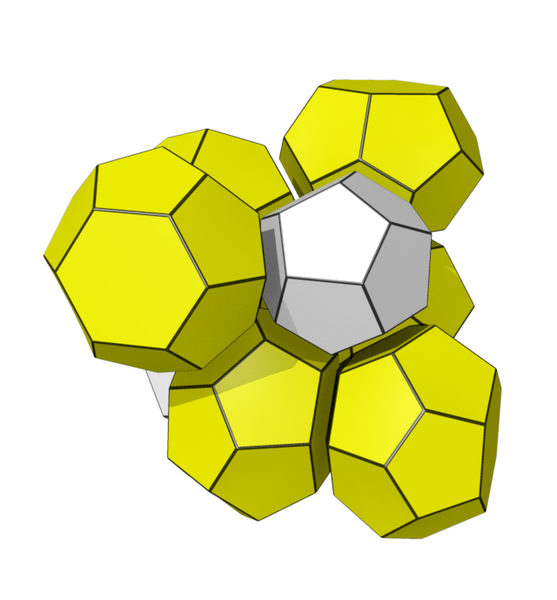
\includegraphics[scale=0.28]{557px-Foam_-_Weaire-Phelan_structure.png}
  \caption{The Phelan-Weaire foam, giving the best known partition of Euclidean space
into cells of equal volume, was constructed with Surface Evolver software.
This foam inspired the bubble design of the Water Cube building in the 2008 Beijing Olympics.
}
\label{fig:PW}
\end{figure}
%[XX Insert Kelvin foam graphic.]
% http://it.wikipedia.org/wiki/File:Foam_-_Weaire-Phelan_structure.png XX wiki graphic,
% permissions probably OK.


\subsection{kissing numbers} % (transcient use section)


\begin{figure}[h!]
  \centering
\includegraphics[scale=0.6]{kissing_number2.jpg}
  \caption{In two dimensions, the kissing number is $6$. In eight dimensions, the answer is $240$.
   The proof certificate was found by linear programming.}
\label{fig:kissing}
\end{figure}

% http://www.cwi.nl/news/2011/siagoptimization-prize-kissing-number-research, graphics source, permissions needed.

In the plane, at most six pennies can be arranged in a hexagon so that they
all touch one more penny placed at the center of the hexagon (Figure~\ref{fig:kissing}).  Odlyzko
and Sloane, solved the corresponding problem in dimension $8$: at most
$240$ nonoverlapping congruent balls can be arranged so that they all
touch one more at the center.  

 Up to rotation, a unique arrangement of
$240$ exists.  To the cognoscenti, the proof of this fact is expressed as one-line certificate:
\[
(t - \frac{1}{2})t^2(t + \frac{1}{2})^2 (t + 1).
\]
% copied from Pfender-Ziegler.
(For an explanation of the certificates, see \cite{PZ}.)
The certificate was produced by a linear programming computer search, but once
the certificate is in hand, the proof is computer-free.

As explained above, six is the {\it kissing number} in two dimensions,
$240$ is the kissing number in eight dimensions. In three dimensions,
the kissing number is $12$.  This three-dimensional problem goes back
to a discussion between Newton and Gregory in 1694, but was not
settled until the 1950s.  A recent computer proof makes an exhuastive
search through nearly 100 million combinatorial possibilities to
determine exactly how much the twelve spheres must shrink to
accommodate a thirteenth~\cite{Musin-Tarasov}.  Bachoc and Vallentin
were recently awarded the SIAG/Optimization prize for their use of
semi-definite programming algorithms to establish new proofs of the
kissing number in dimensions $3,4,8$ and new bounds on the kissing
number in various other dimensions~\cite{BV08}.



\subsection{digression on $E_8$}\label{sec:e8}

It is no coincidence that the calculation of Odlyzko and Sloane works
in dimension $8$.  Wonderful things happen in eight dimensional space
and again in $24$ dimensions.

Having mentioned the $240$ balls in eight dimensions, I cannot resist
mentioning some further computer proofs.  The centers of the $240$ balls
are vectors whose integral linear cominations generate 
a lattice in $\ring{R}^8$, known as the $E_8$ lattice (Figure~\ref{fig:e8}).

There is a packing of congruent balls in eight dimensions that is
obtained by centering one ball at each vector in the $E_8$ lattice,
making the balls as large as possible without overlap.  Everyone
believes that this packing in eight dimensions is the densest
possible, but this fact currently defies proof.  Cohn and Kumar have a beautiful
computer assisted proof that the $E_8$ packing is the densest of all
{\it lattice} packings in $\ring{R}^8$ (and the corresponding result in
dimension $24$ for the Leech lattice).  That is, among all packings
whose centers form a lattice.  The proof is based on the Poisson
summation formula.  Pfender and Ziegler's account of this
computer-assisted proof won the Chauvenet Prize of the MAA for
writing~\cite{PZ}.

%% chauvenet. 2006.
%% http://mathdl.maa.org/mathDL/22/?pa=content&sa=viewDocument&nodeId=3065

\begin{figure}[h!]
  \centering
\includegraphics[scale=0.35]{Dynkin_diagram_E8.png}
  \caption{The $E_8$ lattice is generated by eight vectors in $\ring{R}^8$ whose
mutual angles are $120^\circ$ or $90^\circ$ depending on whether the corresponding
circles are joined by a segment are not.}
\label{fig:e8}
\end{figure}
% http://en.wikipedia.org/wiki/File:Dynkin_diagram_E8.svg, wiki source, XX use probably ok.
%[Insert graphic of $E_8$ Dynkin diagram.]

The $240$ vectors that generate the $E_8$ lattice are the {\it roots}
of a $240+8$ dimensonal Lie group (also called $E_8$); that is, a
differentiable manifold that has the analytic structure of a group.
All simple Lie groups were classified in the nineteenth
century.\footnote{I describe the families over $\ring{C}$.  Each
  complex Lie group has a finite number of further real forms.}  They
fall into infinite families named alphabetically, $A_n$, $B_n$, $C_n$,
$D_n$, with $5$ more exceptional cases that do not fall into infinite
familes $E_6$, $E_7$ $E_8$, $F_4$, $G_2$.  The exceptional Lie
group\footnote{For decades, $E_8$ has stood for the ultimate in
  speculative physics, whether in heterotic string theory or a
  ``theory of everything.''  Last year, $E_8$ took a turn toward the
  real world, when $E_8$ calculations predicted neutron scattering
  experiments with a cobalt niobate magnet~\cite{BGE8}.} of highest
dimension is $E_8$.

The long-term {\it Atlas Project} aims to use computers to determine
all unitary representations of real reductive Lie groups~\cite{Atlas}.
The $19$-member team   focused on $E_8$
first, because everyone respects the formidable $E_8$.  By 2007, a
computer had completed the character table of $E_8$.  Since there are
infinitely many irreducible characters and each character is an
analytic function on (a dense open subset of) the group, it is not
clear without much further explanation what it might even mean for a
computer to output the full character table as a $60$ gigabyte file.  What
is significant about this work is that it brings the computer to bear
on some abstract parts of mathematics that have been traditionally
largely beyond the reach of concrete computational description,
including infinite dimensional representations of Lie groups,
intersection cohomology and perverse sheaves.  Vogan's account of this
computational project was awarded the 2011 Conant Prize of the
AMS~\cite{VE8}.

% (working in seamless harmony??) Vogan's phrase.

%Leeuwen's slides describe how a heavily recursive calculation requiring 160 GB
%of RAM was squeezed into 64 GB RAN. 

% XX Give NYT citation.
% Vogan, The character table for E8.
% E8 paper.
% http://atlas.math.umd.edu/software/
% cite (Marc Leuwen, computational aspects).
% http://atlas.math.umd.edu/talks/cracking-E8.pdf
% from 160 GB to 64 GB.
% http://young.sp2mi.univ-poitiers.fr/~marc/pdf/Zaragoza-E8.pdf

% 60 gb comes from http://atlas.math.umd.edu/talks/boston.pdf
% it also says 77 hours.


While on the topic of computation and representation theory, I cannot
resist a digression into the $P$ versus $NP$ problem, the most
fundamental unsolved problem in mathematics. In my opinion, attempts
to prove $P$ versus $NP$ from the axioms of ZFC are ultimately as
ill-fated as Hilbert's program in the foundations of math (which
nonetheless spurred valuable partial results such as the decision
procedures of Presburger and Tarski), but if I were to place faith
anywhere, it would be in Mulmuley's program in {\it geometric
  complexity theory}.  The program invokes geometric invariant theory
and representation theoretic invariants to tease apart complexity
classes: if the irreducible constituents of modules canonically
associated with two complexity classes are different, then the two
complexity classes are distinct.  In this approach, the determinant
and permanent of a matrix are chosen as the paradigms of what is easy
and hard to compute, opening up complexity theory to a rich
algebro-geometric structure~\cite{Mul11},~\cite{FPNP}.



\subsection{future computer proofs}

Certain problems are natural candidates for computer proof: the Kelvin
problem by the enumeration of the combinatorial topology of possible
counterexamples; the search for a counterexample to the
two-dimensional Jacobian conjecture through the minimal model
program~\cite{Borisov}; resolution of singularities in positive
characteristic through an automated search for numerical quantities
that decrease under suitable blowup; existence of a projective plane
of order $12$ by constraint satisfaction programming; the optimality
proof of the best known packing of regular tetrahedra in three
dimensions~\cite{Chen-2010}; and the Reinhardt conjecture through
nonlinear optimization~\cite{HR11}.  But proceed with caution!
Checking on our zeal for brute
computation, computer-generated patterns can sometimes fail miserably.
For example, Stanley's sequence:
\[
\left\lceil{\frac{2}{2^{1/n} - 1}}\right\rceil- 
\left\lfloor{\frac{2 n}{\log 2}}\right\rfloor,\quad n=1,2,3,\ldots
\]
starts out as the zero sequence, but remarkably first gives a nonzero
value when $n$ reaches $777,451,915,729,368$ and then again when
$n=140,894,092,055,857,794$.
% http://mathoverflow.net/questions/15444/the-phenomena-of-eventual-counterexamples
% http://oeis.org/A129935



%\section{Mathematical Software}

% (Give broad categories and one-line programs. Use ICMS proceedings)

This short survey has almost completely neglected the areas of
mathematical algorithms and software! To survey mathematics in the age
of the Turing machine is a reckless undertaking, especially if it does
not mention the Euclidean algorithm, Newton's method, Gaussian
elimination, fast Fourier transform, simplex algorithm, sorting, and
Sch\"onhage-Strassen.  A starting point for the exploration of mathematical
software is the KNOPPIX/Math, a bootable DVD with over a hundred
 free mathematical software products, including Sage~\cite{HK08}.

\begin{figure}[h!]
\centering
\begin{tabular}{|@{~~}l@{~~}|@{~~}l@{~~}|}
\hline
\TeX & Active-DVI, AUC\TeX, \TeX{}macs, Kile, Whizzy\TeX\\
computer algebra & Axiom, CoCoA4, GAP, Macaulay2, Maxima,\\
&PARI/GP, Risa/Asir, Sage, Singular, Yacas\\
numerical calc&Octave, Scilab, FreeFem++, Yorick\\
visualization& 3D-XplorMath-J, Dynagraph, GANG, Geomview, \\
 &gnuplot, JavaView, K3DSurf\\
geometry& C.a.R, Dr.Geo, GeoGebra, GEONExT, KidsCindy, KSEG\\
programming & CLISP, Eclipse, FASM, Gauche, GCC, Haskell, Lisp\\
&Prolog, Guile, Lazarus, NASM, Objective Caml,\\
&Perl, Python, Ruby, Squeak\\
\hline
\end{tabular}
\caption{A few of the free mathematical programs on the Knoppix/Math DVD}
\end{figure}


\newpage
\section{Automating Proof}

Proof assistants represent the best effort of logicians, computer
scientists, and mathematicians to obtain complete mathematical rigor
by computer.  This section gives a brief introduction to proof
assistants and describes various recent projects that use them.

The first section described various computer calculations in math,
and this section turns to computer reasoning.  I have never been able to
get used to it being the mathematicians who use computers for calculation
and the computers scientists who use computers for proofs!
% I hope the
%situation will change in the future as proof assistants move towards
%widespread adoption!


\subsection{design of proof assistants}

A formal proof is a proof that has been checked at the level of the
primitive rules of inference all the way back to the fundamental
axioms of mathematics.  The number of primitive inferences is
generally so large that it is quite hopeless to construct a formal
proof by hand of anything but theorems of the most trivial nature.
McCarthy and de Bruijn suggested that we program computers to generate
formal proofs from high-level descriptions of the proof.  This
suggestion has led to the development of proof assistants.

% McC and de Bruijn, page 10 of ftp://ftp.cs.ru.nl/pub/CSI/CompMath.Found/wiley.pdf

A {\it proof assistant} is an interactive computer program that enables a user to
generate a formal proof from its high-level description.  The computer code
that implements a proof assistant lists the fundamental axioms
of mathematics and gives procedures that implement each of the rules of logical
inference.  Within this general framework, there are enormous variations
from one proof assistant to the next. The following feature-table is
reproduced from~\cite{wiedijk:17}.  The columns list different proof
assistants, HOL, Mizar, etc.  Since it is the one that I am most familiar with,
my discussion will focus largely on a particular
proof assistant, {\it HOL Light}, which belongs to the {\it HOL} family of
proof assistants. {\it HOL} is an acronym for Higher-Order Logic, which is the underlying
logic of these proof assistants.

Without going into full detail, I will make a few comments
about what some of the features mean.  Different systems can be
commended in different ways: HOL Light for its small trustworthy
kernel, Coq for its powerful type system, Mizar for its extensive
libraries, and Isabelle/HOL for its support and useability.

\bigskip
% http://andrewjpage.com/index.php?/archives/24-Latex-tables-and-rotated-text.html
\noindent
\begin{figure}
\centering
\begin{tabular}{|r|ccccc|ccccc|ccccc|cc|}\hline
~{\it proof assistant}~
&\begin{sideways}HOL\end{sideways}
&\begin{sideways}Mizar\end{sideways}
&\begin{sideways}PVS\end{sideways}
&\begin{sideways}Coq\end{sideways}
&\begin{sideways}Otter/Ivy\end{sideways}
&\begin{sideways}Isabelle/Isar\end{sideways}
&\begin{sideways}Alfa/Agda\end{sideways}
&\begin{sideways}ACL2\end{sideways}
&\begin{sideways}PhoX\end{sideways}
&\begin{sideways}IMPS\end{sideways}
&\begin{sideways}Metamath\end{sideways}
&\begin{sideways}Theorema\end{sideways}
&\begin{sideways}Lego\end{sideways}
&\begin{sideways}Nuprl\end{sideways}
&\begin{sideways}$\Omega$mega\end{sideways}
&\begin{sideways}$B$ method\end{sideways}
&\begin{sideways}Minilog\end{sideways}\\
\hline
small proof kernel (`proof objects')
&+ &- &- &+  &+ &+ &+ &-  &+ &- &+ &-  &+ &- &+ &-  &+ 
\\
calculations can be proved automatically
&+ &- &+ &+  &+ &+ &- &+  &+ &+ &- &+  &+ &+ &+ &+  &+ 
\\
extensible/programmable by the user~
&+ &- &+ &+  &- &+ &- &-  &- &- &- &-  &- &+ &+ &-  &+ 
\\
powerful automation~
&+ &- &+ &-  &+ &+ &- &+  &- &+ &- &+  &- &- &+ &+  &- 
\\
readable proof input files~
&- &+ &- &-  &- &+ &- &+  &- &- &- &+  &- &- &- &-  &- 
\\
\hline
constructive logic supported~
&- &- &- &+  &- &+ &+ &-  &- &- &+ &-  &+ &+ &- &-  &+ 
\\
logical framework~
&- &- &- &-  &- &+ &- &-  &- &- &+ &-  &- &- &- &-  &- 
\\
typed~
&+ &+ &+ &+  &- &+ &+ &-  &+ &+ &- &-  &+ &+ &+ &-  &+ 
\\
decidable types~
&+ &+ &- &+  &- &+ &+ &-  &+ &+ &- &-  &+ &- &+ &-  &+ 
\\
dependent types~
&- &+ &+ &+  &- &- &+ &-  &- &- &- &-  &+ &+ &- &-  &- 
\\
\hline
based on higher order logic~
&+ &- &+ &+  &- &+ &+ &-  &+ &+ &- &+  &+ &+ &+ &-  &- 
\\
based on ZFC set theory~
&- &+ &- &-  &- &+ &- &-  &- &- &+ &-  &- &- &- &+  &- 
\\
large mathematical standard library~
&+ &+ &+ &+  &- &+ &- &-  &- &+ &- &-  &- &+ &- &-  &- 
\\
statement about $\ring{R}$~
&+ &+ &+ &+  &- &+ &- &+  &- &+ &+ &+  &- &- &+ &-  &+ 
\\
statement about $\sqrt{\phantom X}$~
&+ &+ &+ &+  &- &+ &- &-  &- &+ &+ &+  &- &- &+ &-  &- 
\\
\hline
\end{tabular}
\caption{Features of proof assistants}
\label{fig:feature}
\end{figure}

% Permissions needed. XX get permission for table.

\bigskip 




\subsubsection{small proof kernel.} If a proof assistant is used to
check the correctness of proofs, who checks the correctness of the
proof assistant itself?  De Bruijn proposed that the computer code
implementing a proof assistant should be short -- something that
can be checked by hand.  For example, the kernel of the proof
assistant HOL Light is just $430$ lines of very readable computer
code.  The architecture of the system is such that if these $430$
lines are bug free then it is incapable\footnote{I
  exaggerate. Section~\ref{sec:trust} goes into detail about trust in
  computers.} of generating a theorem that hasn't been properly
proved.

\subsubsection{automating calculations.} Mathematical argument
involves both calculation and proof.  The foundations of logic often
specify in detail what constitutes a mathematical proof (a sequence of
logical inferences from the axioms), but downgrade calculation to
second-class status, requiring every single calculation to undergo a
cumbersome translation into logic.  Poincar\'e has drawn a distinction
between verification of individual facts such as $2+2=4$ (which he
says ``leads to nothing'') and what he calls ``real
proofs''~\cite[p.~4]{HPSH}.  This distinction has come to mean the
distinction between the algorithmically solvable and the rest.  If a
proof assistant admits as proof the output from a verified algorithm
(bypassing the expansive translation into logic of each separate
execution of the algorithm), then we say that the {\it Poincar\'e
  principle} holds for that algorithm.  The closely related principle
of {\it reflection} is proof based on the syntactic form of a term,
rather than the term itself~\cite{BFM}.



\subsubsection{constructive logic.} The
law of excluded middle $\phi\lor\lnot \phi$ is accepted in classical
logic, but rejected in constructive logic.  A proof assistant
may be constructive or classical.  A box ({\it A Mathematical Gem}) shows how HOL Light becomes
classical through the introduction of an axiom of choice.

\newpage
\bigskip
\noindent

\framebox{\parbox{4.6in}{ \smallskip \centerline{\it A Mathematical
      Gem -- Proving the Excluded Middle} \smallskip The logic of HOL
    Light is intuitionistic until the axiom of choice is introduced
    and classical afterwards.  By a result of Diononescu~\cite{Bee85}, choice and
    extensionality imply the law of excluded middle (to phi or not to phi):
 \[\phi\lor \lnot\phi.\]

The proof is such a gem that I have chosen to include it as the only
complete proof in this survey paper.  Consider the two sets of booleans
\begin{align*}
P_1 &= \{ x \mid (x = \text{false}) \lor ((x = \text{true}) \land \phi)\}\quad \text{and}\\
P_2  &= \{x \mid (x = \text{true}) \lor ((x = \text{false}) \land \phi)\}.
\end{align*}
The sets are evidently nonempty, because $\false\in P_1$ and $\true\in P_2$.
By choice, we may pick  $x_1\in P_1$ and $x_2\in P_2$; and by the definition of $P_1$ and $P_2$:
\[
(x_1=\text{false})\lor (x_1 = \text{true}),\qquad (x_2=\text{false})\lor (x_2 = \text{true}). 
\]
We may break the proof of the excluded middle into four cases, depending on the
two possible truth values of each of $x_1$ and $x_2$.

{\bf Cases} $(x_1,x_2)=(\true,\true),$ $(x_1,x_2)=(\true,\false)$: By
the definition of $P_1$, if $x_1 = \true$, then $\phi$, so $\phi\lor
\lnot\phi$. 

 {\bf Case} $(x_1,x_2)=(\false,\false)$: Similarly, by the definition
of $P_2$, if $x_2=\false$, then $\phi$, so also $\phi\lor\lnot\phi$.

{\bf Case} $(x_1,x_2)=(\false,\true)$: If $\phi$, then $P_1=P_2$, and
the choices $x_1$ and $x_2$ reduce to a single choice $x_1=x_2$, which
contradicts $(x_1,x_2)=(\false,\true)$.  Hence $\phi$ implies
$\false$; which by the definition of negation gives $\lnot\phi$, so
also $\phi\lor\lnot\phi$.\hfill{\it Q.E.D.}

}}



\newpage


\subsubsection{logical framework.} 
Many different systems of logic arise in computer science.  In some
proof assistants the logic is fixed. Other proof assistants are more
flexible, allowing different logics to be plugged in and played with.
The more flexible systems implement a meta-language, a {\it logical
  framework}, that gives support for the implementation of multiple
logics.  Within a logical framework, the logic and axioms of a proof
assistant can themselves be formalized, and machine
translations\footnote{My Flyspeck project seeks to give a formal proof
  of the Kepler conjecture~\cite{Hales:2005:DSP}. This project is now scattered
  between different proof assistants. Logical
  framework based translations between proof assistants gives me hope that an automated tool may
  assemble the different parts of my project.} can be constructed between
different foundations of mathematics~\cite{IRFF}.

\subsubsection{type theory.}

Approaching the subject of formal proofs as a mathematician whose
practise was shaped by Zermelo-Fraenkel set theory, I first treated
types as nothing more than convenient identifying labels (such real
number, natural number, list of integers, or boolean) attached to terms,
like the 
%hash tags on tweets or the 
PLU stickers on fruit that get peeled
away before consumption.  Types are familiar from programming
languages as a way of identifying what data structure is what.  In the
simple type system of HOL Light, to each term is affixed a unique
type, which is either a primitive type (such as the boolean type
$\op{\it bool}$), a type variable ($A,B,C,\ldots$), or inductively
constructed from other types with the arrow constructor
($A\rightarrow B$, $A\rightarrow (\op{\it bool} \rightarrow C)$,
etc.).  There is also way to create subtypes of existing types.
If the types are interpreted naively as sets, then $x\tc A$
asserts that the term $x$ is a member of $A$, and $f:A\rightarrow B$
asserts that $f$ is a member of $A\rightarrow B$, the set of functions
from $A$ to $B$.

In untyped set theory, it is possible to ask ridiculous questions such
as whether the real number $\pi=3.14\ldots$, when viewed as a raw set,
is a finite group.  In fact, in a random exploration of set theory,
like a monkey composing sonnets at the keyboard, ridiculous questions
completely overwhelm all serious content.  Types organize data on the
computer in meaningful ways to cut down on the static noise in the
system.  The question about $\pi$ and groups is not well-typed and
cannot be asked.  Russell's paradox also disappears: $X \not\in X$ is
not well-typed.  For historical reasons, this is not surprising:
Russell and Whitehead first introduced types to overcome the paradoxes of
set theory, and from there, through Church, they passed into computer
science.


Only gradually have I come to appreciate the signficance of a
comprehensive {\it theory of types}.  The type system used by a proof
assistant determines to a large degree how much of a proof the user
must contribute and how much the computer automates behind the scenes.
The type system is {\it decidable} if there is a decision procedure to
determine the type of each term.

A type system is {\it dependent} if a type can depend on a value of
another type.  For example, Euclidean space $\ring{R}^n$, depends on
its dimension $n$.  For this reason, Euclidean space is most naturally
implemented in a proof assistant as a dependent type.  
In a proof assistant such as HOL Light that does not have dependent types,
extra work is required to Euclidean space.


\subsection{propositions as types}

I mentioned the naive interpretation of each type $A$ as a
set and a term $x\tc A$ as a member of the set.  A quite different
interpretation of types has had considerable influence in the design
of proof assistants.  In this ``terms-as-proofs'' view, a type $A$ represents a
proposition and a term $x\tc A$ represents a proof of the proposition
$A$.  A term with an arrow type, $f:A\rightarrow B$, can be used to to
construct a proof $f(x)$ of $B$ from a proof $x$ of $A$.  In this
interpretation, the arrow is logical implication. 

A further interpretation of types comes from programming languages.
In this ``terms-as-computer-programs'' view, each type is a datatype
in a programming language.  The term $x$ has type $A$ in $x\tc A$, and
$f:A\rightarrow B$ is a computer program $f$ that takes input of type
$A$ and returns a value of type $B$.

By combining the ``terms as proofs'' with the ``terms as computer
programs'' interpretations, we get the famous {\it Curry-Howard
  correspondence} that identifies proofs with computer programs and
identifies each proposition with the type of a computer program. 
For example,  the most fundamental rule of logic,
\[
\frac{A,\quad A\rightarrow B}{B},  \qquad \text{\it(modus ponens)}
\]
(from $A$ and $A\text{-implies-}B$ follows $B$) is identified with the
function application in a computer program; from $x\tc A$ and $f:A\rightarrow B$ we get
$f(x)\tc B$.
 The
Curry-Howard correspondence has been extremely fruitful, with a
multitude of variations, running through a gamut of proof systems in
logic and identifying each with a suitable programming domain.  To follow
the correspondence is to extract an
executable computer program from a mathematical proof.






\subsection{proof tactics}

In some proof assistants, the predominant proof style is a backward style
proof.  The user starts with a {\it goal}, which is a statement to be proved. In
interactive steps, the user reduces the goal to successively
simpler goals until there is nothing left to prove.

Each command that reduces a goal to simpler goals is called a {\it
  tactic}.  For example, in the proof assistant HOL Light, there are
about 100 different commands that are tactics or higher-order
operators on tactics (called tacticals).  Figure~\ref{fig:tactic}
shows the most commonly used proof commands in HOL Light.  The most
common tactic is {\it rewriting}, which takes a theorem of the form
$a=b$ and substitutes $b$ for an occurence of $a$ in the goal.

\bigskip
\noindent
\begin{figure}
\centering
\begin{tabular}{|@{~~}l@{~}|@{~}l@{~}|@{~}c@{~~}|}\hline
\text{\it name}  &~\text{\it purpose} &\text{\it usage}\\
\hline
\text{THEN\dots }   &~\text{combine two tactics into one}   & 37.2\%\\
\text{REWRITE \dots} &~\text{use $a=b$ to replace $a$ with $b$ in goal} & 14.5\%\\
\text{MP\_TAC} &~\text{introduce a previously proved theorem} &4.0\%\\
\text{SIMP\_TAC \dots}&~\text{rewriting with conditionals} & 3.1\%\\
\text{MATCH\_MP\_TAC} &~\text{reduce a goal $b$ to $a$, given a theorem $a\Longrightarrow b$}& 3.0\%\\
\text{STRIP\_TAC} &~\text{(bookkeeping) unpackage a bundled goal} & 2.9\%\\
\text{MESON\_TAC \dots}&~\text{apply first-order reasoning to solve the goal} & 2.6\%\\
\text{REPEAT} &~\text{repeat a tactic as many times as possible} & 2.5\%\\
\text{DISCH\_TAC \dots}&~\text{(bookkeeping) move hypothesis to the assumption list\!\!\!} & 2.3\%\\
\text{EXISTS\_TAC}&~\text{instantiate an existential goal $\exists x\dots$}& 2.3\%\\
\text{GEN\_TAC}&~\text{instantiate a universal goal $\forall x\dots$}& 1.4\%
\\
\hline
\end{tabular}
\caption{A few of the most common proof commands in the HOL Light proof assistant}
\label{fig:tactic}
\end{figure}
\bigskip

In the Coq proof assistant, the tactic systems has been streamlined to
an extraordinary degree by the {\it SSReflect} package, with a small
number of tactics such as the {\it move} tactic to do the bookkeeping,
the {\it have} tactic to do forward reasoning and a rewriting tactic,
{\it rewrite}~\cite{gonISSR},~\cite{gonSSRE}.  It serves as a model of efficiency for other proof
assistants to emulate.  The package also
provides support for exploiting the computational content of proofs,
augmenting logical reasoning with efficient computational algorithms.
%



\subsection{first-order automated reasoning}

Many proof assistants support some form of automated reasoning to
relieve the user of doing rote logic by hand. For example, Table~\ref{fig:tactic}
lists the {\it meson} (an acronym for Loveland's Model Elimination
procedure), which is HOL Light's tactic for automated reasoning~\cite[Sec.~3.15]{Ha09},
~\cite{harrison:meson}.
The various automated reasoning tools are generally {\it first-order}
theorem provers.  The classic resolution algorithm for first-order
reasoning is illustrated in a box ({\it Proof by Resolution}).

\newpage
\bigskip
\noindent

\framebox{\parbox{4.6in}{ \smallskip \centerline{\it Proof by
Resolution} \smallskip 
\parskip=\baselineskip

Resolution is the granddaddy  of automated reasoning
in first-order logic. 
The resolution rule  takes two disjunctions 
\[P\lor A, \qquad  \text{and}\qquad \lnot P' \lor B\] and
concludes \[A'\lor B',\] where $A'$ and $B'$ are the specializations of
$A$ and $B$, respectively, under the most general unifier of $P$ and $P'$.
(Several examples of how this works in practice appear below.)

This box presents a rather trivial example of proof by resolution, to
deduce the easy theorem asserting that every infinite set has a
member.  The example will use the following notation.  Let $\emptyset$
be a constant representing the empty set and constant $c$ representing
a given infinite set. We use three unary predicates $e$, $f$, $i$ that
have interpretations
\[
e(X)~~\text{``$X$ is empty''},
\quad f(X)~~\text{``$X$ is finite''}, 
\quad i(X)~~\text{``$X$ is infinite''}.
\]
The binary predicate $(\in)$ denotes set membership.
Write $u(X)\in X$ when there exists $u\in X$.
We prove $i(c) \Rightarrow (\exists z. z\in c)$ ``an infinite set has a member'' by resolution. 

To argue by contradiction,
we introduce the
hypothesis $i(c)$ and the negated conclusion $\lnot (Z\in c)$ as axioms.
Here are the axioms that we introduce for the deduction.  The axioms have
been preprocessed, stripped of quantifiers, and written as a disjunction of literals.

\bigskip\noindent
\begin{tabular}{lll}
&{\it Axiom}&{\it Description}\\
1.~&$i(c)$~~&Assumption of desired theorem.\\
2.&$\lnot (Z\in c)$~~&Negation of conclusion of desired theorem.\\
3.&$e(X) \lor (u(X)\in X)$~~&A nonempty set has a member.\\
4.&$e(\emptyset)$~~&The empty set is empty.\\
5.&$f(\emptyset)$~~&The empty set is finite.\\
6.&$\lnot i(Y) \lor \lnot f(Y)$~~&A set is not both finite and infinite.\\
7.& $\lnot e(U) \lor \lnot e(V) \lor \lnot i(U) \lor i(V)$~~&Indistinguishability of empty sets.\\
\end{tabular}
\bigskip

Here are the resolution inferences from this list of axioms. The final step obtains the
desired contradiction. 

\bigskip
\begin{tabular}{lll}
{\it }&{\it Inference}&{\it Conclusion}\\
~8.&(resolving 2,3, unifying $X$ with $c$ and $u(X)$ with $Z$)~~~~~&$e(c)$\\
~9.&(resolving 7,8, unifying $U$ with $c$)~~~&$\lnot e(V) \lor \lnot i(c) \lor i(V)$\\
10.&(resolving 1,9)~~~&$\lnot e(V) \lor  i(V)$\\
11.&(resolving 4,10, unifying $V$ with $\emptyset$)~~~&$i(\emptyset)$\\
12.&(resolving 6,11, unifying $Y$ with $\emptyset$)~~~&$\lnot f(\emptyset)$\\
13.&(resolving 12,5)~~~&$\perp$\\
\end{tabular}
\bigskip
{{\it Q.E.D.}}

}}

\newpage


Writing about first-order automated reasoning, Huet and Paulin-Mohring
\cite{Coq} describe the situation in the early 1970s as a
``catastrophic state of the art.''  ``The standard mode of use was to
enter a conjecture and wait for the computer's memory to exhaust its
capacity.  Answers were obtained only in exceptionally trivial
cases.'' %\footnote{-tr. T. Hales}
%\footnote{Le mode standard d'utilisation \'etait de rentrer sa conjecture et
%d'attendre que la m\'emoire de l'ordinateur soit satur\'ee.  Seulement dans des cas
%exceptionnellement triviaux une r\'eponse \'etait obtenue.''
They go on to describe numerous developments (Knuth-Bendix, LISP,
rewriting technologies, LCF, ML, Martin-L\"of type theory, NuPrl,
Curry-Howard correspondence, dependent types, etc.) that led up to the
Coq proof assistant.  These developments led away from first-order
theorem proving with its ``thousands of unreadable logical
consequences'' to a highly structured approach to theorem proving in Coq.


First-order theorem proving has developed significantly over the years
into sophisticated software products.  They are no longer limited to
``exceptionally limited cases.''  There are now many different
software products that compete in an annual competition (CASC), to see
which can solve difficult first-order problems the fastest.  The LTB
(large theory batch) division of the competition includes problems
with thousands of axioms~\cite{PSST}.  Significantly, this is the same order of
magnitude as the total number of theorems in a proof assistant.  What
this means is that a first-order theorem provers have reached the
stage of development that they might be able to give fully automated
proofs of new theorems in a proof assistant, working from the full
library of previously proved theorems.

% Ref. PSST=CASC_ desktop Thackmac.

\subsubsection{sledgehammer.}

The Sledgehammer tactic is Paulson's implementation of this idea of full automation in
the Isabelle/HOL proof system~\cite{Paar}.  As the name `Sledgehammer' suggests,
the tactic is all-purpose and powerful, but demolishes all higher
mathematical structure, treating every goal as a massive unstructured
problem in first-order logic.  If $L$ is the set of all theorems in
the Isabelle/HOL library, and $g$ is a goal, it would be possible hand
off the problem $L\Longrightarrow g$ to a first-order theorem
prover.  However, success rates are dramatically improved, when the
theorems in $L$ are first assessed by heuristic rules for their likely
relevance for the goal $g$, in a process called {\it relevance
  filtering}. 
% The heuristic relevance filtering rules are currently
%very simple rules, such as a theorem is in $L$ is more likely to be
%relevant for the proof of $g$, if $L$ and $g$ have some constants in
%common.  
This filtering is used to reduce $L$ to an axiom set $L'$ of a
few hundred theorems that are deemed most likely to prove $g$.

The problem $L'\Longrightarrow g$ is stripped
of type information, converted to a first-order, and fed
 in parallel into several first-order theorem provers.  
%According to B\"ohme and Nipkow, on average
%``Running each of the 3 provers for 5 [seconds] yields the same M-success rate
%(44\%) as running the most effective one [Vampire] for 120 [seconds].''
 ``B\"ohme and Nipkow \cite{Boehme-Nipkow-IJCAR10} have demonstrated that
running three different [first-order] theorem provers (E, SPASS and
Vampire) for five seconds solves as many problems as running the
best theorem prover (Vampire) for two full minutes.  It would be
better to utilise even more theorem provers'' 
\cite{Paar}.
% Paulson, paar. Desktop Thackmac.
When luck runs in your favor, one of the first-order theorem provers finds
a proof.

The reconstruction of a
formal proof from a first-order proof can encounter hurdles.  For one thing, when type
information is stripped from the problem (which is done to improve
performance), soundness is lost.  ``In unpublished work by Urban,
MaLARea [a machine learning program for relevance ranking] easily
proved the full Sledgehammer test suite by identifying an
inconsistency in the translated lemma library; once MaLARea had found
the inconsistency in one proof, it easily found it in all the
others'' \cite{Paar},~\cite{UrM}. 
% Paulson, paar.
% cite: MaLARea: a metasystem for automated reasoning in large theories, Urban
%Even when the first-order proof is valid, Hurd and Paulson found that
%in most cases, the first-order proofs were not explicit enough to permit a
%reconstruction of
%a formal proof.
%``Hurd [7] had noticed that
%the proofs delivered by automatic theorem provers (Gandalf, in his
%case) were not detailed and explicit enough. We made the same
%discovery [14] (in the case of SPASS), and despite considerable
%efforts, were only able to reconstruct a handful of
%proofs.'' % Paulson, paar.
Good results have been obtained in calling the first-order prover repeatedly to find a smaller
set of axioms $L''\subset L'$ that imply the goal $g$. A manageably
sized set $L''$ is then passed to the metis tactic\footnote{Metis is a
  15K line program in SML that replaces the meson prover described
  above~\cite{Metis}.} in Isabelle/HOL, which constructs
a formal proof $L''\Longrightarrow g$ from scratch.

%Instead, once a first-order proof of the goal $g$ is found with axiom
%set $L'$.  The theorem prover is repeatedly called on smaller and
%smaller axiom sets $L''\subset L'$ until a small set of axioms is
%identified that prove the goal $g$.  Ideally, this process reduces the
%size of the axiom set from the hundreds in $L'$ to a set $L''$ of only
%a few.  In other words, the first-order prover is used as nothing more
%than a massive relevance filter, to identify a small set of theorems
%in the Isabelle/HOL library that imply the goal $g$.  The manageably
%sized set $L''$ is then passed to the metis tactic\footnote{Metis is a
%  15K line program in SML that replaces the meson prover described
%  above~\cite{Metis}.} in Isabelle/HOL, which independently constructs a proof
%$L''\Longrightarrow g$.  

%T http://www.gilith.com/software/metis/notes.html  Metis.

B\"ohme and Nipkow \cite{Boehme-Nipkow-IJCAR10} have tested the success rates of the
sledgehammer tactic on a large test suite.  They took 1240 proof goals
that appear in several diverse theories of the Isabelle/HOL system and
ran sledgehammer on all of them. The results are truly
astounding. The success rate (of obtaining fully reconstructed proofs
by metis inside the proof assistant) when three different first-order
provers run for two-minutes each was 48\%.  The proofs of these same
goals by hand might represent years of human labor, now fully
automated through a single new tool.
% XX check years claim. 

% http://isabelle.in.tum.de/~nipkow/pubs/ijcar10.pdf Nipkow.

Sledgehammer has led to a new style of theorem proving, in which the
user is primarily responsible for stating the goals.  In the final
proof script, there is no explicit mention of sledgehammer.  Metis
proves the goals, with sledgehammer operating silently in the
background to feed metis with whatever theorems it needs.
For example, a typical proof script might contain  lines such as \cite{Paar}
\[
\begin{array}{ll}
\text{{\bf hence} ``$x \subseteq \text{space}~M$''}\\
\text{~~~{\bf by} (metis sets into space lambda system sets)}&
\end{array}
\]
The first line is the goal provided the user. The second line has been
automatically inserted into the proof script by the system, with
theorems {\tt sets, into, \dots} selected by Sledgehammer.


% Paulson (3-years paar, Desktop, Thackmac.)




\subsection{computation in proof assistants.}

One annoyance of formal proof systems is that the number of theorems
is overwhelming.   At the last count, the proof system HOL Light had about $14,000$
theorems and nearly a thousand procedures for proof construction.
Larger developments, such as Mizar, have about twice as many theorems.
Good search tools have somewhat relieved the burden of locating theorems
that have already been verified in a system.  However, as the formal proof
systems continue to grow, it becomes ever more important to be able to 
use theorems without mentioning them by name.


% 933 indexed help entries.  14,030 indexed theorems June 12, 2011, with flyspeck loaded.

As an example of a feature which commendably reduces the burden of
memorizing long lists of theorem names, I mention the {REAL\_RING} command in
HOL Light\footnote{
  Cezary Kaliszyk's benchmarks suggest that the Gr\"obner basis algorithm in 
the proof assistant Isabelle
  runs about twenty times faster than that of HOL Light.
%% ref. CICM 2011 presentation by C.K.
}, 
which is capable of proving any system of equalities and
inequalities that holds over an arbitrary integral domain.  For
example, I can give a one-line formal proof of an isogeny $(x_1,y_1)
\mapsto (x_2,y_2)$ of elliptic curves: if we have
\begin{align*}
y_1^2 &= 1 + a x_1^2 + b x_1^4,\\
x_2 y_1&=x_1,\\
y_2 y_1^2&=(1 - b_1^4),\\
y_1&\ne 0
\end{align*}
then $(x_2,y_2)$ satisfies
\[
y_2^2 = 1 + a' x_2^2 + b' x_2^4,
\]
where $a' = -2a$ and $b' = a^2 - 4b$.  In the proof assistant, 
%the automated formal proof of
%this identity takes $0.2$ seconds on my laptop, and 
the input of the
statement is as economical as what I have written here. We expect computer
algebra systems to be capable of checking identities like this, but to
my amazement, I found it {\it easier} to check this isogeny in HOL
Light than to check it in {\it Mathematica}.

The algorithm works in the following manner.  A universally
quantified system of equalities and inequalities holds over all integral
domains if and only if it holds over all fields.  
By putting the formula
in conjunctive normal form, it is enough to prove a finite number of
identities of the form:
\begin{equation}\label{eqn:q}
(p_1(x)=0) \lor \cdots \lor (p_n(x)=0) \lor (q_1(x)\ne 0) \lor\cdots\lor (q_k(x)\ne 0).
\end{equation}
An element in a field is zero, if and only if it is not a unit.  Thus we may
rewrite each equality $p_i(x)=0$ as an equivalent inequality $1-p_i(x)z_i\ne 0$.
Thus, without loss of generality, we may assume that $n=0$; so that all disjuncts
are inequalities.  The formula (\ref{eqn:q}) is logically equivalent to
\[
(q_1(x) =0) \land \cdots \land (q_k(x) = 0) \Longrightarrow \text{false}.
\]
In other words, it is enough to prove that 
the ideal $I=(q_1,\ldots,q_n)$ has no common zero.  For this,
we may use Gr\"obner bases  to prove that $1\in I$, to certify that
there is no common zero.  



%% REAL_RING `a' = &2 * a /\ b' = a*a - &4 * b /\ x2 * y1 = x1 /\ y2 * y1 pow 2 = &1 - b * x1 pow 4 /\ y1 pow 2 = &1 + a * x1 pow 2 + b * x1 pow 4 /\ ~(y1 = &0) ==> y2 pow 2 = &1 - a' * x2 pow 2 + b' * x2 pow 4`;;

\smallskip

Another praiseworthy project is Kaliszyk and Wiedijk's implementation
of a computer algebra system on top of the proof assistant HOL Light.
It combines the ease of use of computer algebra with the rigor of
formal proof~\cite{kaliszyk_p04_calc}.  Even with its notational
idiosyncracies (\verb!&! and \verb!#! as a markers of real numbers,
\verb!Cx! as a marker of complex numbers, \verb!ii! for $\sqrt{-1}$,
and \verb!--! for unary negation), it is the kind of product that I
can imagine finding widespread adoption by mathematicians. A session
with the system is shown in Figure~\ref{fig:kw}.

\begin{figure}
\begin{verbatim}
 In1 := (3 + 4 DIV 2) EXP 3 * 5 MOD 3 
Out1 := 250 
 In2 := vector [&2; &2] - vector [&1; &0] + vec 1 
Out2 := vector [&2; &3] 
 In3 := diff (diff (\x. &3 * sin (&2 * x) + &7 + exp (exp x))) 
Out3 := \x. exp x pow 2 * exp (exp x) + exp x * exp (exp x) + -- &12 * sin (&2 * x) 
 In4 := N (exp (&1)) 10 
Out4 := #2.7182818284 + ... (exp (&1)) 10 F 
 In5 := 3 divides 6 /\ EVEN 12 
Out5 := T 
 In6 := Re ((Cx (&3) + Cx (&2) * ii) / (Cx (-- &2) + Cx (&7) * ii)) 
Out6 := &8 / &53 
\end{verbatim}
\caption{Interaction with a formally verified computer algebra system.}
\label{fig:kw}
\end{figure}
% \lambda -> \,   /\ -> \land.
% XX need permissions.  Copied from kaliszyk_p04_calc


\subsection{overloaded lemmas}

% How to make ad hoc proof automation less ad hoc. Gonthier et al.

Theorems retain various advantages over automated proof procedures.  
As mentioned above, the list of all theorems can be easily searched by name or by
matching subterm.  We can search for the fundamental theorem of arithmetic, but we
have no way to search for the procedure {\it REAL\_RING}.  We learn its existence and
usage by reading the user manual.  If a user contributes a new proof procedure, we
have no systematic way to find out about it.

Every theorem is self-documenting; the statement of the theorem and
its supporting definitions give me all that I need to use it. As much
as mathematicians take pride in understanding the proofs of theorems
they cite, this is not a logical necessity.  In classical logic, this
property of theorems is called proof irrelevance.  By contrast, the
meaning of a proof procedure is ultimately the body of computer code
that implements it.  If we are lucky, the code is clean and
well-documented.  When out of luck, we experiment and guess from their
names what the procedures
{\it sledgehammer}, {\it blast}, and {\it meson} can do.

Finally, theorems are composable in ways that proof procedures are not.  They
can be used in simplification, rewrites, and model elimination (meson).

In a move toward making proof assistants more useable, Gonthier et al.
have developed {\it overloaded lemmas}~\cite{gonHoc}.  These are objects that have
the look and feel of theorems (in fact they are theorems), but behave
like an automated proof procedure, giving the best of both worlds.
A simple example is the overloaded lemma
\[
\text{for all natural numbers}~m~n.~m+n  = \text{\it computed-answer.}
\]
When we instantiate the variables $m$ and $n$ to $1$ and $2$ we get
the theorem $1+2=3$, and when we instantiate the variables to $2$ and
$3$ we get the theorem $2+3=5$.  The point is that instantiation
triggers a procedure that computes the sum $m+n$ and fills the open
slot {\it computed-answer} with the result.  They show that by playing
games with dependent types,
instantiation of variables can trigger arbitrarily complex procedures
that fill the open slots of a theorem.



\begin{figure}[h!]
\centering
\begin{tabular}{l l l l l}
\hline
Year\hspace{0.5em} &Theorem\hspace{8em} &Proof System\hspace{2em}  &Formalizer\hspace{3em} &Traditional Proof\\ [0.5ex]
\hline \\
1986 &First Incompleteness &Boyer-Moore   &Shankar &G\"odel \\
1990 &Quadratic Reciprocity&Boyer-Moore &Russinoff &Eisenstein\\
1996 &Fundamental - of Calculus &HOL Light &Harrison &Henstock\\
2000 &Fundamental - of Algebra &Mizar &Milewski    &Brynski\\ % email tchales@gamil.com, Aug 17 from Milewski mentions  Brynski.
2000 &Fundamental - of Algebra &Coq &Geuvers et al.   &Kneser\\
2004 &Four Color &Coq &Gonthier &Robertson et al.\\
2004 &Prime Number &Isabelle &Avigad et al. &Selberg-Erd\"os\\
2005 &Jordan Curve  &HOL Light &Hales &Thomassen \\
2005 &Brouwer Fixed Point &HOL Light &Harrison &Kuhn \\
2006 &Flyspeck I &Isabelle &Bauer-Nipkow &Hales \\
2007 &Cauchy Residue &HOL Light &Harrison &classical \\
2008 &Prime Number &HOL Light &Harrison &analytic proof \\
% 2008 &Flyspeck II &Isabelle &Obua &Hales \\
 [1ex]
\hline
\end{tabular}
\caption{Examples of Formal Proofs}
\label{table}
\end{figure}

% XX link table to text somewhere.


\subsection{formalization of finite group theory}



The Feit-Thompson theorem, or odd-order theorem as it is sometimes
called, is one of the most significant theorems of the twentieth
century.  (For his work, Thompson was awarded the three highest forms
forms of recognition in the mathematical world: the Fields Medal, the
Abel Prize, and the Wolf Prize.)  The Feit-Thompson theorem states
that every finite simple group has even order, except for cyclic
groups of prime order.  Although the statement is very simple, the
proof is extremely technical and runs about 250 pages. It relies on
numerous other theorems in group and character theory.  The
Feit-Thompson theorem was the key ingredient in the classification of
all finite simple groups, a monumental undertaking that engulfed an
entire generation of group theorists.

% Peterfalvi, Thomas (2000), Character theory for the odd order theorem, London Mathematical Society Lecture Note Series, 272, Cambridge University Press, ISBN 978-0-521-64660-4, MR1747393

% Bender, Helmut; Glauberman, George (1994), Local analysis for the odd order theorem, London Mathematical Society Lecture Note Series, 188, Cambridge University Press, ISBN 978-0-521-45716-3, MR1311244

From a strictly mathematical point of view, the most significant
current development in the world of formal proofs is Gonthier's team
project to formalize the Feit-Thompson theorem.\footnote{As of January
  2011, the project was about half complete and progressing rapidly,
  having completed the formalization of \cite{BG94} but not yet
  \cite{P00}.}  Why does this formalization project have particular
historical significance?

(1) It works out the formal architecture of abstract algebraic
structures.\footnote{Analogous hierarchies of algebraic structures
  appear in systems such as OpenAxiom, MathScheme, and Isabelle; while some of these
  hierarchies are elaborate, none have delved to Gonthier's formal
  depth.}  Of course, the formal architecture of abstract algebraic
structures has already been worked out by a long line of
mathematicians, including Noether, van der Waerden, and Bourbaki.
Nevertheless, we may hope that the reimplementation of abstract
algebra by computer may soon come to represent the single largest
transformation of the subject since category theory.  I can imagine a
future generation of textbooks in abstract algebra for math majors
that are based on a formal implementation.

% XX http://www.open-axiom.org/,
% XX http://www.cas.mcmaster.ca/research/mathscheme/ (Carette)

%  Earlier formalization projects in abstract algebra did not go much beyond Sylow's first theorem.

 Significantly, it shows how to get multiple abstract structures
to work coherently together in a formal setting.  As Gonthier
correctly observes, when it comes to the formal development of
abstract algebra, ``the problem is not much in capturing the semantics
of each individual construct but rather in having all the concepts
working together well.'' % p14. Mod. Form.

(2) People in the world of formal proofs tend to be drawn into
formalizing results that have elegant self-contained proofs and to
follow the published proofs as closely as possible.  Some even feel a
duty to remain faithful to the published text.  The theorems tend to
be ones that have been worked over by mathematicians for a century or
so.  By contrast, Gonthier is drawn to major theorems with a
forbidding allure, and uses the power of computation to tame them.

The definition of a finite group in Coq is similar to the textbook definition,
expressed in types and structures (Figure~\ref{fig:group}).
\bigskip

\begin{figure}
{

\obeylines\tt
Structure~finGroupType~Type~:= FinGroupType \{
~~~element~:>~finType;
~~~~~~~1~:~element;
~~~~~~\hskip0.8mm ${}^{-1}$~:~element $\to$ element;
~~~~~~~*~:~element $\to$ element $\to$ element;
~~~unitP~:~$\forall\,x,~1*x = x$;
~~~~invP~:~$\forall\,x,~x^{-1} * x = 1$;
~~~~mulP~:~$\forall\,x_1~x_2~x_3,~ x_1 * (x_2 * x_3) = (x_1 * x_2) * x_3$
\}.

}
\caption{The structure for finite groups.}
\label{fig:group}
\end{figure}

\smallskip

It declares a finite type called {\tt element} that is the group
carrier or domain.  The rest of the structure specifies a left-unit
element $1$, a left-inverse ${}^{-1}$ and an associative binary
operation $( * )$.  It is an exercise in group theory to check that
the axioms imply that the left-unit is a two-sided unit and that the
left-inverse is a two-sided inverse.

Other aspects of Gonthier's recent work can be found at
\cite{gonPFSF}, \cite{gonPMS}, \cite{gonMF}, \cite{gonC}.


Along different lines, a particularly elegant organization of abstract
algebra and category theory is obtained with type
classes~\cite{SpE11}.

\subsection{homotopy type theory}

The simple type theory of HOL Light is adequate for real
analysis, where relatively few types are needed -- one can go quite
far with natural numbers, real numbers, booleans, functions between
these types, and a few functionals.  However, the dependent type
theory of Coq is better equipped than HOL Light for the hierarchy of
structures (groups, rings, modules, fields, etc.) of abstract algebra.
But even Coq's type theory is showing signs of strain in dealing with
abstract algebra.  For instance, an unpleasant limitation of Coq's
theory of types is that it lacks the theorem of extensionality for
functions: if two functions take the same value for every argument, it
{\it does not} follow that the two functions are equal.\footnote{HOL Light
  posits extensionality as one of its three mathematical axioms: function extensionality, choice,
  and infinity.}.  Gonthier's gymnastics to solve the problem of
function extensionality in the context of the Feit-Thompson theorem
are found in ~\cite{XX}.

A lack of a theorem of extensionality for functions is an indication
that equality in type theory is misconceived.  In recent years, a
promising new research area {\it homotopy type theory} has exploded
onto the scene, which turns to homotopy theory and higher categories
as models of type theory~\cite{htt}.  In fact, it is quite natural to
interpret a dependent type (viewed as a family of types parametrized
by a second type) topologically as a fibration (viewed as a family of
fibers parametrized by a base space)~\cite{AW09}. Voevodsky took the
homotopical notions of equality and equivalence and translated them
back into type theory, obtaining the {\it univalence axiom} of type
theory, which posits when types are equivalent~\cite{VV11}.  One
sanity check of the univalence axiom is that it implies the theorem of
extensionality for functions.  Another promising sign for computer
theorem-proving applications is that the new axiom appears to preserve
the computable aspects of type theory (unlike for instance, the axiom
of choice which makes non-computable choices)~\cite{LH11}.  Type
theory might infuse back into homotopy theory as well, as with the
recent type-theoretic proof that the higher homotopy groups are
abelian.






% XX Gonthier, Types, Agda, HOL,




\subsection{a need for formal verification}

Let's take the longsided view that the longest proofs of the last century 
are of insignificant complexity compared to what awaits.
Why whould we limit our creative endeavors to $10,000$ page proofs when we have tools
that allow us to go to a million pages or more?  So far at least, no computer proof
has defied human understanding.  But eventually, we will have to content ourselves
with fables that approximate the content of a computer proof in terms that humans
can comprehend.




\subsection{language of mathematics}

Turing's great theoretical achievements were to delineate what a
computer can do in the concept of a universal Turing machine, to
establish limits to what a computer can do in his solution to the {\it
  Entscheidungsproblem}, and yet to advocate nonetheless that
computers might imitate all intelligent activity. It remains a
challenging research program:
% (and a stunnng metynomy): 
to show
that one limited branch of mathematics, computation, might stand for
all mathematical activity.

In the century since Turing's birth, the computer has become so
ubiquitous and the idea of computer as brain so commonplace that it
bears repeating that we must still think very long and hard about how
to construct a computer that can imitate a living, thinking
mathematician.  As a first step toward imitation, we need a computer
that understands the language of mathematics.

%at a time when the
%meaning of the word computer was just starting to shift from a dreary
%human occupation to a mechanical device.

\bigskip

Ganesalingam's thesis \cite{Gan09}, \cite{Gan10} is the most
significant linguistic study of the language of mathematics to date.
Ganesalingam was awarded the 2011 Beth Prize for the best dissertation
in Logic, Language, or Information.  Although this research is still
at an early stage, it suggests that the mechanical
translation that the mechanical translation of mathematical prose into
formal computer syntax that faithfully represents the semantics is a
realistic hope for the not-to-distant future.

% http://www.cl.cam.ac.uk/news/2011/07/mohan-ganesalingam-awarded-beth-prize/

% http://people.pwf.cam.ac.uk/mg262/GanesalingamMdis.pdf The Language of Mathematics.

The linguistic problems surrounding the language of mathematics differ
in various ways  from those of say standard English.  A
mathematical paper introduces new definitions and new notations as it
progesses, whereas in English, the meaning of words is generally
fixed from the outset.  Mathematical writing freely mixes
English with symbolic expressions.  At the same time, mathematics is
self-contained in a way that English can never be; to understand
English is to understand the world.  By contrast, the
meaning in a carefully written mathematical
paper is determined by Zermelo Fraenkel set theory (or your
favorite foundational system).

Ganesalingam's analysis of notational syntax is general enough to treat quite
general mixfix operations generalizing 
infix (e.g. +), postfix (e.g. factorial !), and prefix ($\cos$).  
He analyzes subscripted infix
operators (such as a semidirect product $H\rtimes_\alpha N$),
multi-symboled operators (such as the three-symboled $[~:~]$ operator
for the degree $[K:k]$ of a field-extension), prefixed words
($R$-module), text within formulas $\{(a,b) \mid a \text{~is a factor
  of~} b\}$, unusual script placement ${}^LG$, chained relations
$a<b<c$, ellipses $1+2+\cdots+n$, contracted forms $x,y\in\ring{N}$,
and exposed formulas (such as ``for all $x>0$, \dots'' to mean ``for
all $x$,~if $x>0$, then \dots'').

The thesis treats what is called the formal mode of the language of
mathematics -- the language divested all the side-remarks.  The
syntax is treated as a context-free grammar, and the semantics are
analyzed with a variant of Discourse Representation Theory, which in
my limited understanding is something very similar to first-order
logic; but different in one significant aspect: it provides a theory
of pronoun references; or put more formally, a theory of what may be
the ``legitimate antecedent for anaphor.''

A major issue in Ganesalingam's thesis is the resolution of ambiguity.
For example, in the statement
\begin{equation}\label{eqn:P}
P \text{\it ~is prime}
\end{equation}
 the term `prime' may mean prime number, prime ideal, or prime
manifold.  His solution is to attach type information to terms (in the
sense of types as discussed above).  The reading of (\ref{eqn:P})
depends on the type of $x$, a number, a subset of a ring, or a
manifold.  In this analysis, resolution of ambiguity becomes a task of
a type inference engine.  

Because of the need for type information, Ganesalingam raises
questions about the suitability of Zermelo-Fraenkel set theory as the
ultimate semantics of mathematics.  A number of formal-proof
researchers have been arguing in favor of typed foundational systems
for many years.  It is encouraging that there is  remarkable
convergence between Ganesalingam's linguistic analysis and say
Gonthier's analysis of abstract algebra in Coq. For example, in both
camps we find ellipses (aka big operators), mixfix operators, type
inference, missing argument inference mechanisms, etc.





\subsection{what proof assistants need}


\def\princ#1{\smallskip\hfill\break\smallskip\centerline{\it #1\hfill}}

\princ{1. ``Don't use manual procedures.''~\cite{XX}}

  The same book articulates the {\it DRY} principle:
\princ{2. ``Don't repeat yourself.''}
% Andy Hunt and Dave Thomas, The Pragmatic Programmer.

Current proof assistants are a long way from this principle.  After
all, an entire formal proof is nothing but an embellished repetition
of a mathematical text.  Everyone actively involved in proof
formalization experiences an incessant barrage of problems that have
been solved multiple times before and that other users will have to
solve multiple times again, because the solutions are not systematic.
The noise to signal ratio in these products is intolerably high.

%Today I needed in HOL Light the $i$th component of a vector $\v\in \ring{R}^n$. Some languages $v.i$, or $v[i]$, but I had forgotten that it was $v\$i$.  How do I look it up.  How did I look it up last time?  How did other users look it up.

A related principle is not to say too much.  
Proof assistants should follow Halmos's guideline of writing style to ``omit
any computation which is routine. \dots Merely indicate the starting point,
describe the procedure, and state the outcome''~\cite{Halmos}.  The routine
should be automated and hidden behind the curtain.

\princ{3. Abstract mathematical 
structures produce the best code.~\cite{XX}} % Carette XX

Mathematicians  turn to abstraction for a reason: to weed out
extraneous detail.  This applies to computer code and mathematical
reasoning alike.

``Math has a lot of structure; use it.'' (Carette)
% ``Very abstract mathematical formulations help produce the best code.''
% Carette et al. XX http://www.cas.mcmaster.ca/~carette/publications/pepm28p-carette.pdf  (Gem of a paper.)

\princ{4. Do not jumble the construction, maintenance, and presentation
of proofs.}

The construction of formal proofs from a mathematical text is an extremely
arduous process.  For example, I have estimated that the formalization of a single
mathematical proof, the proof of the Kepler conjecture, would take about twenty
years of highly-skilled labor.  Wiedijk's benchmark is that formalization
of a single page of texbook mathematics requires about one week of labor.

I often hear proposals that would increase the labor needed to
formalize a proof, often backed by goals such as ease of maintenance,
elegance of presentation, and pedagogy.  The most common of these are
proposals to make a formal proof scripts more closely resemble a
printed mathematical text.\footnote{To explain the concept of {\it
    separation of concerns}, Dijkstra tells the story of an old
  initiative to create a new programming language that failed
  miserably because the designers felt that the new language had to
  look just like {\it FORTRAN} to gain broad acceptance. ``The proper
  technique is clearly to postpone the concerns for general acceptance
  until you have reached a result of such a quality that it deserves
  acceptance.'' \cite{XX}} %  Dijks, Scientific Thought 
 To me, this is
akin to asking digital watches to have hands, phones to have rotary
dials, or digital cameras to make shutter sounds.  Better to avail
ourselves of automation that was not available in the day of paper
proofs, and to create new mathematical styles suited to the medium.
For example, one style of formal proof construction might look like a
session with computer-aided design (CAD) tool, another style like
functional programming, and yet another like an interaction with Gmail
where an assumption list replaces the inbox.

% XX http://www.cs.utexas.edu/users/EWD/ewd04xx/EWD447.PDF Dijkstra, Sci. Thought.

Let the research into formal proof construction focus on the most
pressing issue as a separate concern: reducing the time and skill it
takes a user to construct a formal proof from a pristine mathematical
text.

Formal proof transformation should be an entirely independent line of
research that starts with a formal proof script and produces its many
byproducts: refactored proofs, proof scripts optimized for execution
time, translations into other proof assistants, natural language 
translations, natural language abstracts, probabalistically checkable
proofs, searchable metadata extracts, and data mines.

% XX Give many references. XX Log. Frameworks Sean's friend on transl.
% Refactoring (Ian), 
% PCP (cite XX, Jerus.).


%If people still letminute hands,

%Separate construction of formal proofs, maintenance, and presentation
%aspects.  Too much focus is on presentation.  I envision proof
%construction software more like a computer-aided design (CAD)
%system than a word processor.  Too many peole are fixated on the
%proof script as natural language text metaphor.


XX The interaction should be a ``control interface,'' deterministic and guidable.
Suddent changes in state are difficult for the user.




\subsection{formalization challenges}

For a long time, proof formalization technology was unable to advance beyond
the mathematics
of the $19$th century, picking classical gems
such as the Jordan curve theorem, the prime number theorem, or
Dirchlet's theorem on primes in arithmetic progressions.  With
Gonthier's work on the Feit-Thompson theorem, formalization has risen
to a new level, by taking on the work of a Field's medalist.

At this level, there is an abundant supply of mathematical theorems to
choose from.  A Dutch research agenda document
lists the formalization of Fermat's Last Theorem as the first in a
list of ``Ten Challenging Research Problems for Computer
Science.''~\cite{Berg}.  Hesselink predicts that this one
formalization project alone will take about ``fifty years, with a very
wide margin.''
% http://www.cs.rug.nl/~wim/fermat/wilesEnglish.html 
Small pieces of the proof of Fermat, such as class field theory, the
Langlands-Tunnell theorem, or the arithmetic theory of elliptic curves
would be a fitting starting point.  The aim is to develop
technologies until formal verification of theorems
becomes routine at the level of Atiyah-Singer index theorem,
Perelman's proof of the Poincar\'e conjecture, the Green-Tao theorem
on primes in arithmetic progression, or Ng\^o's proof of the
fundamental lemma.


\subsection{a general problem solver}

Starting from the early days of Newell, Shaw, and Simon's experiments, researchers
have dreamed of a general-purpose mechanical problem solver.  Generations later,
after untold trials, it remains an unwavering dream.  Among the many
proposals is Kurzweil's three-part approach to general problem solving:
\begin{enumerate} 
\item State your problem in precise terms.
\item Map out the contours of the solution space by traversing it
  recursively, within the limits of available computational resources.
\item Unleash an evolutionary algorithm to configure a neural net to
  tackle the remaining leaves.
\end{enumerate}
He concludes, ``And if all of this doesn't work, then you have a
difficult problem indeed''~\cite{Ku99}.  Yes, indeed we do!  Some day,
energy and persistence will conquer.



\newpage
\section{Issues of Trust}\label{sec:trust}

We all have first-hand experience of the bugs and glitches of
software.  We exchange stories when computers run amok.  Science
recently reported the story of a textbook ``The Making of a Fly'' that
was on sale at Amazon for more than 23 million dollars~\cite{Sci11}.  The
skyrocketing price was triggered by an automated bidding war between
two sellers, who let their algorithms run unsupervised.  The textbook's author,
Berkeley professor Peter Lawrence, said he hoped that the price would
reach ``a billion.''

%% cite Science, Vol 332, 6 May 2011. "The \$23 milllion textbook"

An overpriced textbook on the fly is harmless, except for students who
have it as a required text.  But what about the Flash Crash on Wall
Street that brought a 600 point plunge in the Dow Jones in just 5
minutes at 2:41 pm on May 6, 2010?  According to the New York Times \cite{NYT2010}, the flash
crash started when a mutual fund used a computer algorithm ``to sell
\$4.1 billion in futures contracts.''  The algorithm was designed to
sell ``without regard to price or time.\dots [A]s the computers of the
high-frequency traders traded [futures] contracts back and forth, a
`hot potato' effect was created.''  When computerized traders backed
away from the unstable markets, share prices of major companies
fluctuated even more wildly. ``Over 20,000 trades across more than 300
securities were executed at prices more than 60\% away from their
values just moments before'' \cite{SEC2010} Throughout the crash,
computers followed algorithms to a T, to the havoc
of the global economy. 

% http://en.wikipedia.org/wiki/2010_Flash_Crash
% 2:41-2:46pm time from the NYT graphic.
%T http://www.nytimes.com/2010/10/02/business/02flash.html
%T http://sec.gov/news/studies/2010/marketevents-report.pdf, ``Findings Regarding the Market Events of May 6, 2010'' (SEC etc.) REPORT OF THE STAFFS OF THE CFTC AND SEC TO THE JOINT ADVISORY COMMITTEE ON EMERGING REGULATORY ISSUES , Sept 10, 2010.
 


\subsection{mathematical error}

Why use computers to verify mathematics?  The simple answer is that
carefully implemented proof checkers make fewer errors than 
mathematicians (excepting J.-P. Serre).

Incorrect proofs of correct statements are so abundant that they are
impossible to catalogue.  Kempe's claimed proof of the four-color
theorem stood for more than a decade before Heawood refuted
it~\cite[p.~115]{Mac}.  ``More than a thousand false proofs [of
Fermat's Last Theorem] were published between 1908 and 1912
alone''~\cite{Corry}.  Ralph Boas, former executive editor of Math
Reviews, once remarked that proofs are wrong ``half the
time''~\cite{Aus}.  Many published theorems are like the hanging chad
ballots of the 2000 U.S. presidential election, with scrawls too
ambivalent for a clear yea or nay.  Euclid gave us a method, but even
he erred in the proof of the very first proposition of the Elements
when he assumed without proof that two circles, each passing through
the other's center, must intersect.  The concept that is needed to
repair the gap in Euclid's reasoning is an intermediate value theorem.
This defect in Euclidean geometry was not remedied until Hilbert's
`Foundations of Geometry.'  One mathematician even proposed to me that a
new journal is needed that unlike the others %should be established, distinguished from the others by
only publishes reliable results.

% XX Half the time, Auslander 

Examples of widely accepted proofs of false or unprovable statements
show that our methods of proof-checking are far from perfect.    Lagrange
thought he had a proof of the parallel postulate, but had enough doubt
in his argument to withhold it from publication.  In some cases,
entire schools have become sloppy, such as the Italian school of
algebraic geometry or real analysis before the revolution in rigor
towards the end of the nineteenth century.  Plemelj's 1908 accepted
solution to Hilbert's 21st problem on the monodromy of linear
differential equations was refuted in 1989 by Bolibruch.  Auslander
gives the example of a theorem\footnote{The claim was that every
  homogeneous plane continuum is a simple closed curve.}  published by
Waraskiewicz in 1937, generalized by Choquet in 1944, then refuted
with a counterexample by Bing in 1948~\cite{Aus}.  Another
example\footnote{I would like to thank J. Manfredi for this example.}
is the approximation problem for Sobolev maps between two
manifolds~\cite{Bethuel}, which contains an faulty proof of an
incorrect statement.  The corrected theorem appears in \cite{Hang}.
Such examples are so plentiful that a wiki
page has been set up to classify them, with references to much longer discussions
at Math Overflow~\cite{WikiPIP},~\cite{Over1}, ~\cite{Over2}.

% XX http://en.wikipedia.org/wiki/List_of_published_incomplete_proofs
% XX http://mathoverflow.net/questions/35468
% XX http://mathoverflow.net/questions/879
% XX ``Details are in the book The Riemann-Hilbert Problem by Anosov
% and Bolibruch (Vieweg-Teubner 1994), and a nice popular recounting
% of the story is in Ben Yandell's The Honors Class (A K Peters
% 2002).'' Math Overflow.

Theorems that are calculations or enumerations are especially prone to
error.  Feynman laments, ``I don't notice in the morass of things that something, a
little limit or sign, goes wrong.\dots I have mathematically proven to myself
so many things that aren't true.''
%I'm lousy at proving things -- I always make a mistake 
%\dots And 
% So I always have to check with calculations; and
%\dots I'm very poor at calculations -- I always get the wrong answer''
\cite[p.~885]{FeCo}. Elsewhere, Feynman describes two teams of
physicists who carried out a two-year calculation of the electron
magnetic moment and independently arrived at the same predicted value.
When experiment disagreed with prediction, the discrepancy
was eventually traced to an arithmetic error made by the physicists,
whose calculations were not so independent as originally
believed~\cite[p.~117]{FQED}.  Pontryagin and Rokhlin erred in computing stable
homotopy groups of spheres.  Little's tables of knots from 1885
contains duplicate entries that went undetected until 1974.  In
enumerative geometry, in 1848, Steiner counted $7776$ plane conics
tangent to $5$ general plane conics, when there are actually only
$3264$.  One of the most persistent blunders in the history of mathematics
has been the misclassification of convex Archimedean polyhedra.  Time and again,
the pseudorhombicuboctahedron has been overlooked or illogically excluded from
the classification~\cite{Gr11}.


% [XX Graphic pseudorhombo]

% XX Pont in overflow, Rokhlin in wiki.
% XX Pont in Ioan Mackenzie James, History of Topology p 567.
% XX http://mathoverflow.net/questions/879 , calc examples.
% XX give graphic from overflow.


% XX http://mathoverflow.net/questions/35468
% XX http://mathoverflow.net/questions/879

%  K. Kuperberg gives the example of Lickorish.


% XX Lagrange http://mathdl.maa.org/images/upload_library/22/Ford/Grabiner3-18.pdf








\subsection{In HOL Light we trust}

To what extent can we trust theorems certified by a proof assistant
such as HOL Light?  There are three various aspects to this question.
Is the underlying logic of the system consistent?  Are there any
programming errors in the implementation of the system?  Can a devious
user find ways to create theorems in ways that circumvent the logic of
the system?  Are the underlying compilers, operating system, and
hardware reliable?

Formal methods represent the best cumulative effort of
logicians, computer scientists and mathematicians over the decades and
even over the centuries to create a trustworthy foundation for the
practice of mathematics, and by extension, the practics of science and
engineering.  

\subsection{a network of mutual verification}

John Harrison
%, in a gem of a paper, 
repeats the classical question
{\it ``Quis custodiet ipsos custodes''} -- who guards the
guards~\cite{HaSelf}?  How do we prove the correctness of the prover
itself?  In that paper, he proves the consistency of the HOL Light
logic and the correctness of its implementation in computer code.  He
makes this verification in HOL Light itself!  To skirt G\"odel's
theorem, which implies that HOL Light -- if consistent -- cannot prove
its own consistency, he gives two versions of his proof.  The first
uses HOL Light to verify a weakened version of HOL Light that does not
have the axiom of infinity.  The second uses a HOL Light with a
strengthened axiom of infinity to verify standard HOL Light.


Recently, Mark Adams has developed his own implementation of HOL
(called HOL Zero).  His system has the ability to mechanically import
proofs that were developed in any proof assistant in the HOL
family~\cite{Adams}.  He imported Harrison's verification of HOL
Light, to obtain a HOL Zero verification of HOL Light.  You see where
this is going.  As mechanical translation capabilities are developed
for proof assistants, it becomes possible for different proof
assistants to share consistency proofs, similar to the way that
different axiomatic systems give relative consistency proofs of one
another.  We are headed in the direction of knowing that if the logic
or implementation of one proof assistant has an error, then all other major
proof assistants must fall with it. Other self-verification projects
are Coq in Coq (Coc) and ACL2 in ACL2 (Milawa) ~\cite{Bar98}, ~\cite{Dav09}.

\subsection{hacking HOL}

Of course, every formal verifcation project is a verification of an
abstract model of the computer code, the computer language, and its
semantics.  In practice, there are gaps between the abstract
model and reality.

  
This leaves open the possibility that a hacker might find ways to
create an unauthorized theorem; that is a theorem generated by some
means other than the rules of inference of HOL Logic?  Indeed, there
are small openings that a hacker can exploit.\footnote{For example,
  strings are mutable in Objective CAML, which allows theorems to
  maliciously altered.  Also, Objective CAML has {\it object magic},
  which is a way to defeat the type system.  These vulnerabilities
  and all other vulnerabilities that I know
  would be detected during translation of the proof from HOL Light to
  HOL Zero.}  Adams maintains a
webpage of known vulnerabilities in his system and offers a cash
bounty to anyone who uncovers a new vulnerability.

These documented vulnerabilities need to be kept in perspective.  They
lie at the fringe of the most reliable software products ever
designed. Proof assistants are used verify the correctness of chips
and microcode~\cite{FoxArm6}, operating system kernels~\cite{seL4}, 
compilers~\cite{CC}, safety-critical software such as aircraft
guidance systems, security protocols, and mathematical theorems that
defeat the usual refereeing process.  

Some take the view that nothing short of absolute certainty in
mathematics gives an adequate basis for science.  Poincar\'e was less
exacting\footnote{``Il est donc inutile de demander au calcul plus de pr\'ecision
qu'aux observations; mais on ne doit pas non plus lui en demander moins.''}, 
% from the introduction of the book.
only demanding the imprecision of calculation not to exceed
 experimental error~\cite{HPMC}.  As Harrison puts it, 
``a foundational death spiral adds little value''~\cite{harrison-pm}.


% cite Harrison's Principia slides.

%XX Trust via type system, closed off by modules, implemented in a small
%kernel of 400 lines.


\subsection{soft errors}\label{sec:soft}

Mathematicians often bring up the ``cosmic ray argument'' against the use
of computers in math.  Let's look at the underlying science.

A soft error in a computer is a transcient error that cannot be
attributed to permanent hardware defects nor to bugs in software.  
Hard errors -- errors that can be attributed to a lasting hardware failure --
also occur, but at rates that are ten times smaller than
soft errors~\cite{MW04}.
%% cite: Ritesh Mastipuram and Edwin C Wee, Cypress Semiconductor -- EDN, September 30, 2004 (on hard drive).
Soft errors come from many sources. A
typical soft error is caused by cosmic rays, or rather by the shower
of energetic neutrons they produce through interactions in the earth's
atmosphere.  A nucleus of an atom in the hardware can capture one of
these energetic neutrons and throw off an alpha particle, which
strikes a memory circuit and changes the value stored in memory.  To
the end user, a soft error appears as a gremlin, a seemingly
inexplicable random error that disappears when the computer is rebooted and
the program runs again.

As an example, we will calculate the expected
number of soft errors in one of the mathematical calculations of
Section~\ref{sec:e8}.  The Atlas Project calculation of
the $E_8$ character table was a $77$ hour calculation that required
$64$ gigabytes RAM~\cite{AtlasSlides}.  Soft errors rates are generally measured in units
of failures-in-time (FIT). One FIT is defined as one error per $10^9$
hours of operation.
%The soft error rate of a memory device is typically in the range 1000
%to 5000 FIT per Mbit \cite{White Paper}.
% http://www.tezzaron.com/about/papers/soft_errors_1_1_secure.pdf
If we assume a soft error rate of $10^3$ FIT per Mbit, (which is a
typical rate for a modern memory device operating at sea
level\footnote{The soft error rate is remarkably sensitive to
  elevation; a calculation in Denver produces about three times more
  soft errors than the same calculation on identical hardware in Boston.}
\cite{WP}),
% 3 x in Mastipuram and Wee, EDN article.
 then we would expect there to be about $39$ soft
errors in memory during the calculation:
\[
\frac{10^3 \text{~FIT}}{1\text{~Mbit}} \cdot 64 \text{~GB} \cdot 77\text{~hours} =
\frac{10^3 \text{~errors~}}{10^9\text{~hours~}\text{Mbit}} \cdot
({64\cdot 8\cdot 10^3 \text{~Mbit}}) \cdot 77\text{~hours~} 
\approx 39.4 \text{~errors}.
\]
This example shows that soft errors can be a realistic concern in
mathematical calculations.

In software that has been thoroughly debugged, soft errors become the
most significant source of error in computation.  Although there are
numerous ways to reduce soft errors with methods such as error-correcting
codes, hardware redesign carries an economic cost.  In fact, soft errors are on
the rise through miniaturization: a smaller circuit generally has a lower
capacitance and responds to less energetic alpha particles than a larger
circuit.

Soft errors are depressing news in the ultra-reliable world of proof
assistants.  Alpha particles rain on perfect and imperfect software
alike.  In fact (as JH has pointed out to me), because the number of
soft errors is proportional to the length of a calculation, by being
slow and methodical, the probability of a soft error during a
calculation inside a proof assistant can be much higher than the
probability when done outside.  
%For example, the calculation of a
%double precision floating point approximation to $\sqrt{2}$ with
%interval arithmetic takes about XX flops (or floating-point
%operations).
%\begin{equation}
%1.4 < \sqrt{2} < 1.42 XX.
%\end{equation}
%The formal proof of these inequalities in a proof assistant (HOL
%Light) requires about $10^n$ XX times longer (and thus incurs $10^n$
%times more soft errors) than the interval arithmetic calculation.
Soft errors especially become a issue in a formal proof project that
makes intensive floating-point calculations.
%\footnote{This includes my
%  Flyspeck project, which will include the formalization of a
%  floating-point calculation that take about $12$ hours to run outside the
%  proof assistant and several orders of magnitudes longer inside the proof assistant.}

Soft errors and susceptibility to hacking
have come to be more than a nuisance to me.  They alter my
philosopical views of the foundations of mathematics.  I am a
computational formalist -- a formalist who admits physical
limits to the reliability of any verification process, whether by hand
or machine.  These limits taint even the simplest theorems, such as
our ability to verify that $1+1=2$ is a consequence of a set of
axioms.  One rogue alpha particle brings all my schemes of
perfection to nought.  %No matter how hard I try to reach formal 
%perfection in my mathematical proofs, the stray alpha particle meddles.  
The rigour of
mathematics and the reliability of technology are mutually dependent;
math to provide ever more accurate models of science, and technology
to provide ever more reliable execution of mathematial proofs.

\newpage
\section{Concluding Remarks}


To everyone who has made it this far in my essay,  I
highly recommend MacKenzie's book \cite{Mac}.  It written by a
sociologist with a fine sensitivity to mathematics.  The author
received the Robert K. Merton Award of the American Sociological
Association in 2003 for this book.

A fascinating account of the history of higher-order logic appears in
\cite{Gor}.  A few years ago, a special issue of the Notices of the
AMS presented a general introduction to formal
proofs~\cite{Hales:2008:formal},~\cite{Harrison:2008:formal},
~\cite{gonthier:2008:formal}, ~\cite{Wiedijk:2008:formal}.  I also particularly
recommend the body of research papers by Harrison, Gonthier, and
Carette.



\bigskip

I thank J. Urban, J. Carette and J. Harrison 
for some conversations that influenced the ideas of this article.




\raggedright
\bibliographystyle{amsalpha} % was plain %plainnat
\bibliography{/Users/thomashales/Desktop/googlecode/flyspeck/latex/bibliography/all}


\bigskip
\noindent
\svninfo





\end{document}

